In this section, we consider a set of examples in which the functionality of the \texttt{MPT-Calculator} is demonstrated. Note that these examples have been run with NGSolve 6.2.2004 if running with a different versions the user may obtain different meshes, due to this the meshes used to produce the results have been included in the VolFiles folder. We start with the case of a sphere.
\subsection{Sphere}\label{sectSphereSweeps}
For the case where $B$ is a sphere of unit radius and $\alpha B$ is a sphere of radius $\alpha=0.01 \text{m}$ we shall create three different simulations, the first is a simulation consisting of a single frequency, the second a full order frequency sweep and the third a frequency sweep implementing the POD. All of these sphere examples are created using the \texttt{sphere.geo} file, shown in Figure \ref{fig:SweepSphere}, where $\Omega$ is chosen to be a ball of radius 200 containing the object $B$, $\sigma_*=6\times 10^6\text{ S/m}$ and $\mu_*=1.5\mu_0$.
\begin{figure}[H]
\begin{center}
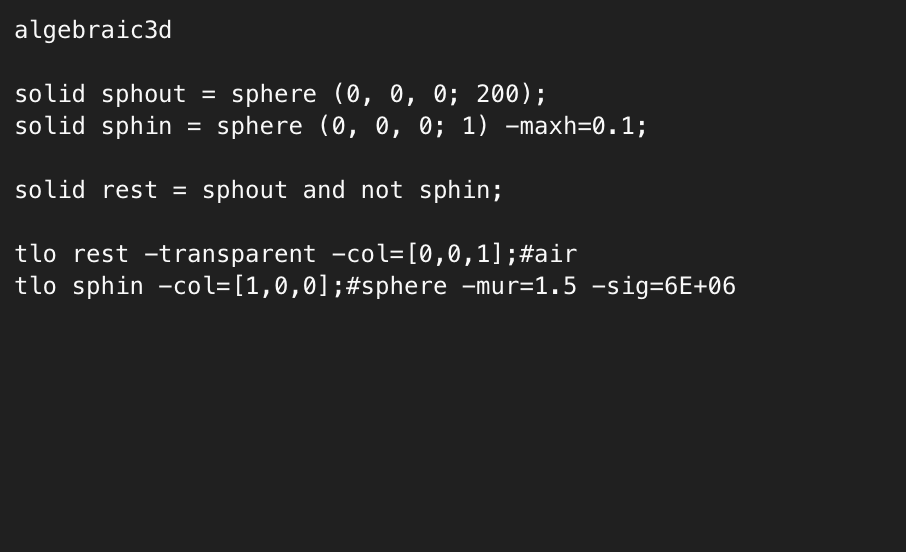
\includegraphics[width=0.5\textwidth]{Figures/SweepSphere.png}
\caption{Image displaying the \texttt{Sphere.geo} file used in all of the sphere frequency sweep examples in Section \ref{sectSphereSweeps}.}\label{fig:SweepSphere}
\end{center}
\end{figure}
\noindent
We start our examples session with a simulation of the sphere described in Figure \ref{fig:SweepSphere} for a single frequency.
\subsubsection{Single frequency sweep for a sphere}
To set up this simulation, we used the \texttt{sphere.geo} file shown in Figure \ref{fig:SweepSphere} along with the inputs displayed in Figure \ref{fig:SphereSingleInputs}.
\begin{figure}[H]
$$\begin{array}{ccc}
\includegraphics[width=0.3\textwidth, keepaspectratio]{Figures/SphereMain} & 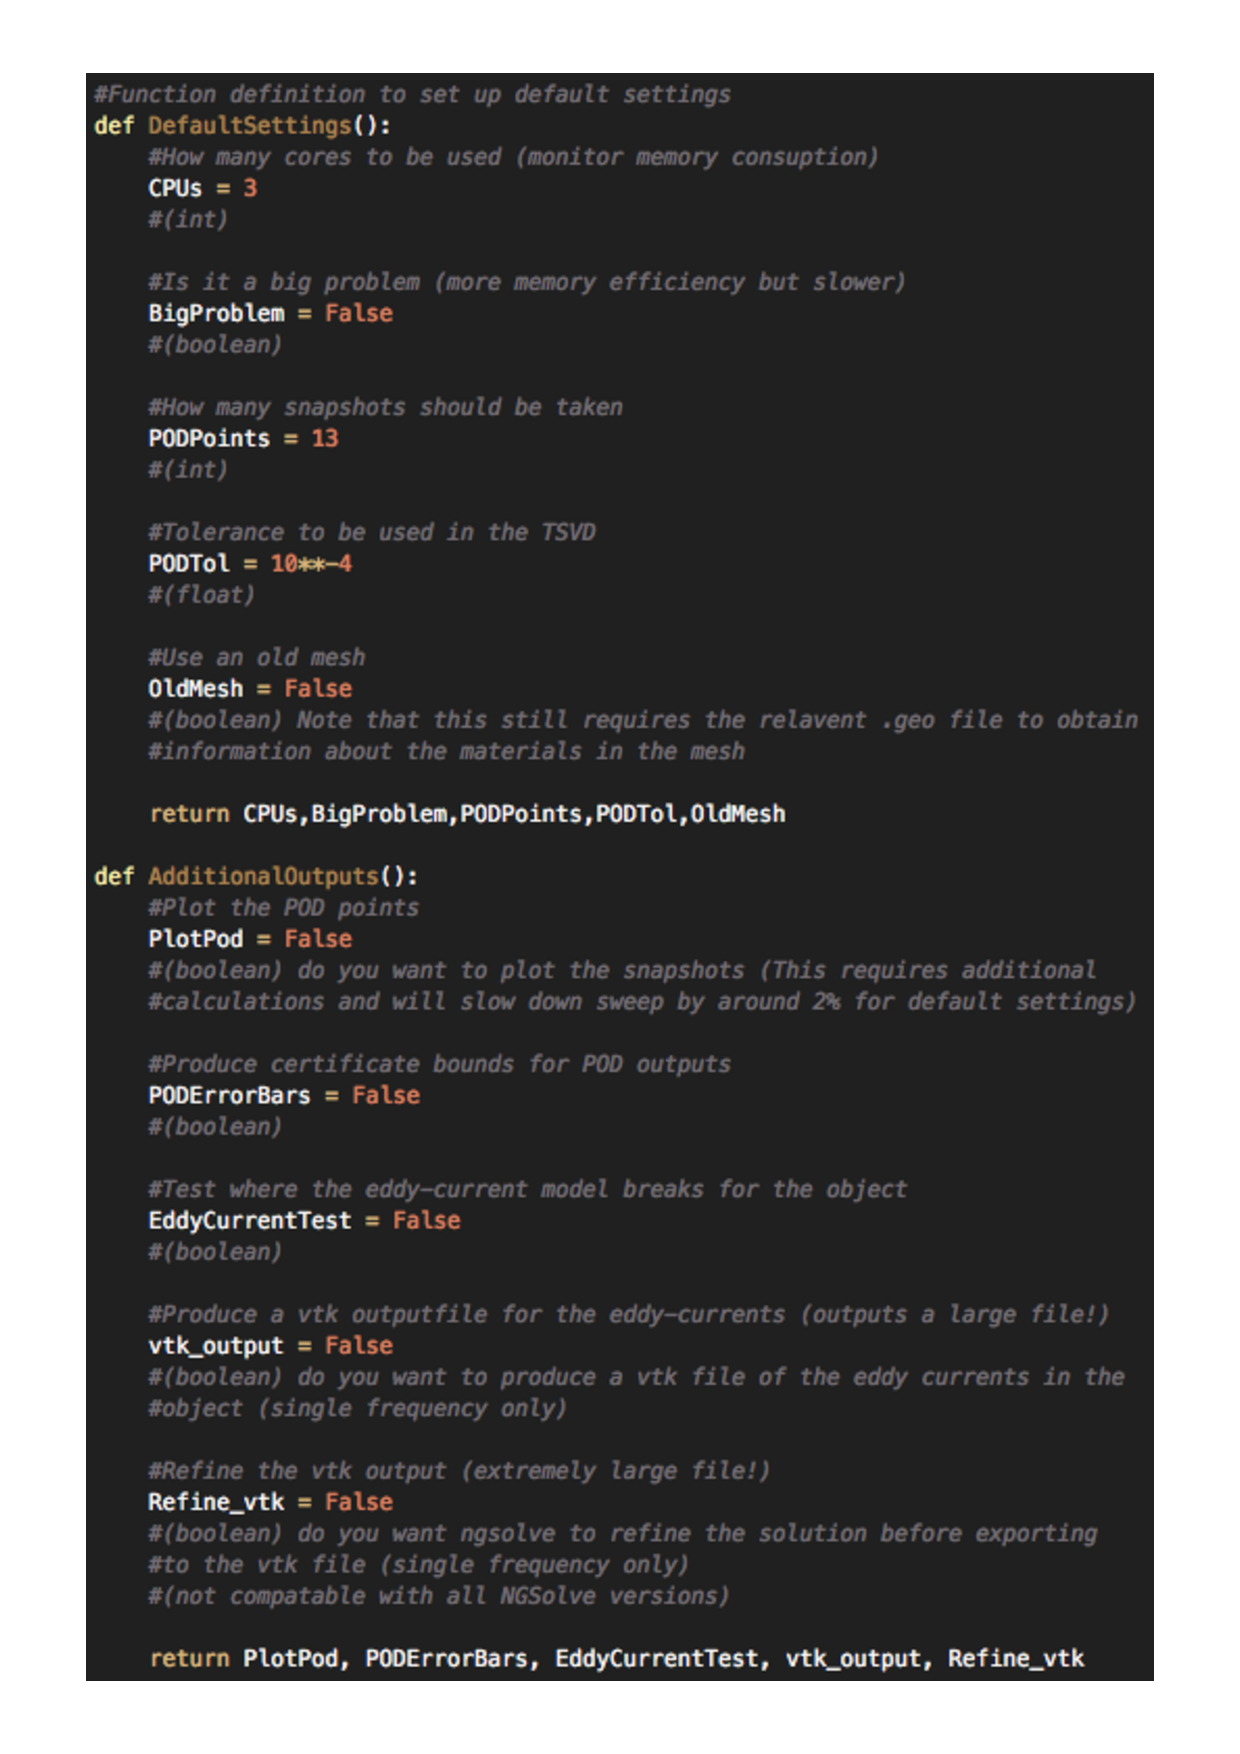
\includegraphics[width=0.3\textwidth, keepaspectratio]{Figures/SphereSettingsTop} & 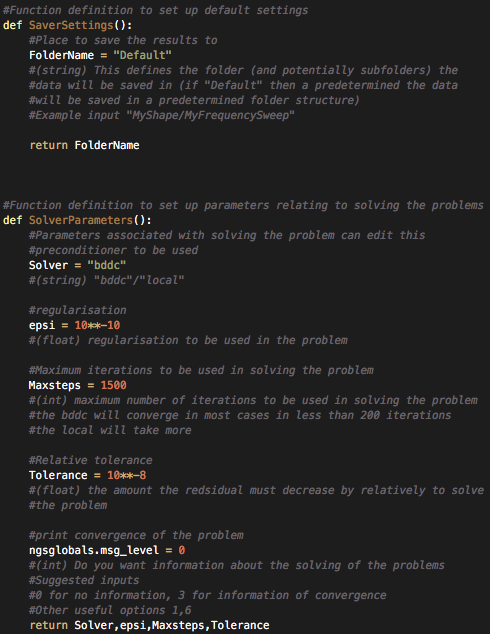
\includegraphics[width=0.3\textwidth, keepaspectratio]{Figures/SphereSettingsBottom}\\
\textrm{\footnotesize{(a) An image of \texttt{main.py}.}} & \textrm{\footnotesize{(b) Top of \texttt{Settings.py}.}} & \textrm{\footnotesize{(c) Bottom of \texttt{Settings.py}.}}
\end{array}$$
%\begin{figure}\label{LogvsLin}
\caption{Images displaying the inputs for the single frequency sweep for a sphere (a) image of the inputs in \texttt{main.py} (b) image of the inputs in the top of \texttt{Settings.py} (c) image of the inputs in the bottom of \texttt{Settings.py}.}
\label{fig:SphereSingleInputs}
\end{figure}
\noindent
These inputs for \texttt{main.py} and \texttt{Settings.py} have been summarised in Table \ref{tab:SphereSingleInputs}. As  \texttt{Single = True} the following variables are not used: \texttt{Start = 1}, \texttt{Finish = 8}, \texttt{Points = 81}, \texttt{Pod = False}, \texttt{PODPoints = 13}, \texttt{PODTol = 10**-4}, \texttt{PlotPod = False} and \texttt{PODErrorBars = False}, hence, their values are arbitrary. 
%\begin{table}[H]
%\begin{center}
%\begin{tabular}{!\vrule l!\vrule l!\vrule l!\vrule}
%\hline
%\texttt{Geometry = "sphere.geo"} & \texttt{Pod = False} & \texttt{EddyCurrentTest = False}\\\hline
%\texttt{alpha = 0.01} & \texttt{MultiProcessing = True} & \texttt{vtk\_output = False}\\\hline
%\texttt{MeshSize = 2} & \texttt{CPUs = 3} & \texttt{Refine\_vtk = False}\\\hline
%\texttt{Order = 3} & \texttt{BigProblem = False} & \texttt{FolderName = "Default"}\\\hline
%\texttt{Start = 1} & \texttt{PODPoint = 13} & \texttt{Solver = "bddc"}\\\hline
%\texttt{Finish = 8} & \texttt{PODTol = 10**-4} & \texttt{epsi = 10**-10}\\\hline
%\texttt{Points = 81} & \texttt{OldMesh = False} & \texttt{Maxsteps = 1500}\\\hline
%\texttt{Single = True} & \texttt{PlotPod = False} & \texttt{Tolerance = 10**-8}\\\hline
%\texttt{Omega = 133.5} & \texttt{PODErrorBars = False} & \texttt{ngsglobals.msg\_level = 0}\\\hline
%\end{tabular}
\begin{table}[H]
\begin{center}
\large{\texttt{main.py}}\normalsize{ }\\\vspace{0.2cm}
\begin{tabular}{!\vrule p{4.5cm}!\vrule p{4.5cm}!\vrule p{4.5cm}!\vrule}
\hline
\texttt{Geometry = "sphere.geo"} & \texttt{alpha = 0.01} & \texttt{MeshSize = 2}\\\hline
\texttt{Order = 3} & \texttt{Start = 1} & \texttt{Finish = 8}\\\hline
\texttt{Points = 81} & \texttt{Single = True} &\texttt{Omega = 133.5}\\\hline
\end{tabular}\\
\begin{tabular}{!\vrule p{4.5cm}!\vrule p{4.5cm}!\vrule}
\texttt{Pod = False} & \texttt{MultiProcessing = True}\\\hline
\end{tabular}
\\\vspace{0.5cm}\large{\texttt{Settings.py}}\normalsize{ }\\\vspace{0.2cm}
\begin{tabular}{!\vrule p{4.5cm}!\vrule p{4.5cm}!\vrule p{4.5cm}!\vrule}
\hline
\texttt{CPUs = 3} & \texttt{BigProblem = False} & \texttt{PODPoints = 13}\\\hline
\texttt{PODTol = 0.0001} & \texttt{OldMesh = False} & \texttt{PlotPod = False}\\\hline
\texttt{PODErrorBars = False} & \texttt{EddyCurrentTest = False} & \texttt{vtk\_output = False}\\\hline
\texttt{Refine\_vtk = False} & \texttt{FolderName = "Default"} & \texttt{Solver = "bddc"}\\\hline
\texttt{epsi = 1e-10} & \texttt{Maxsteps = 1500} & \texttt{Tolerance = 1e-08}\\\hline
\end{tabular}\\
\begin{tabular}{!\vrule p{4.5cm}!\vrule}
\texttt{ngsglobals.msg\_level = 0}\\\hline
\end{tabular}\caption{A table summarising the inputs for the simulation of the sphere with for a single frequency.}\label{tab:SphereSingleInputs}
\end{center}
\end{table}
\noindent
This means our interest lies in computing the characterisation for $ \alpha B = 0.01 B$ at a frequency of $\omega = 133.5 \text{rad/s}$.
Furthermore, the inputs led to a mesh of 29170 elements and a discretisation of $p=3$. On a 2012 iMac with a 2.9 GHz quad core i5 processor with 16 GB 1600 MHz DDR3 memory the computation takes 1 minute and 37 seconds using $3$ CPUs and results in the following for the $\mathcal{N}^0$ and $\mathcal{M}$,
\begin{align*}
\mathcal{N}_{hp}^0 = \left(\begin{array}{ccc}
1.80\times10^{-6} & 6.06\times10^{-14} & 1.89\times10^{-15}\\
6.06\times10^{-14} & 1.80\times10^{-6} & 9.55\times10^{-14}\\
1.89\times10^{-15} & 9.55\times10^{-14} & 1.80\times10^{-6}
\end{array}\right),
\end{align*}
\begin{align*}
\mathcal{M}_{hp} = \left(\begin{array}{ccc}
1.79\times10^{-6}+6.97\times10^{-8}\rm{i} & 5.85\times10^{-14}+6.61\times10^{-15}\rm{i} & -3.53\times10^{-15}+2.23\times10^{-14}\rm{i}\\
5.85\times10^{-14}+6.61\times10^{-15}\rm{i} & 1.79\times10^{-6}+6.97\times10^{-8}\rm{i} & 9.06\times10^{-14}+3.18\times10^{-14}\rm{i}\\
-3.53\times10^{-15}+2.23\times10^{-14}\rm{i} & 9.06\times10^{-14}+3.18\times10^{-14}\rm{i} & 1.79\times10^{-6}+6.97\times10^{-8}\rm{i}
\end{array}\right).
\end{align*}
The exact tensors for this object are known to be diagonal and multiple of identity~\cite{LedgerLionheart2018,Wait1951}. Specifically $(\mathcal{N})_{ii} = 1.80 \times 10^{-6} $ and $(\mathcal{M})_{ii} =  1.79 \times 10^{-6} +6.97 \times 10^{-8} \im $ to 2dp. By repeatably performing $h$ or $p$ refinement, the off diagonal terms tend to $0$ and the diagonal entries of $\mathcal{M}_{hp}$ and  $\mathcal{N}_{hp}$ to their exact values according to the convergence curves presented in Figure \ref{fig:hprefinement}. In this case, the relative error $\| \mathcal{M}- \mathcal{M}_{hp} \|_F / \|\mathcal{M}  \|_F = 2.72 \times 10^{-6}$. We also find the computed eigenvalues to be
\begin{align*}
\lambda(\mathcal{N}^0+\mathcal{R}) = \left(\begin{array}{c}
1.79\times10^{-6}\\1.79\times10^{-6}\\1.79\times10^{-6}
\end{array}\right),\quad
\lambda(\mathcal{I}) = \left(\begin{array}{c}
6.97\times10^{-8}\\6.97\times10^{-8}\\6.97\times10^{-8}
\end{array}\right).
\end{align*}
We next consider the example of a full order frequency sweep once again for the sphere described by the \texttt{.geo} file in Figure \ref{fig:SweepSphere}.
\subsubsection{Full order frequency sweep for a sphere}
A frequency sweep is now performed for the sphere described by the \texttt{sphere.geo} file in Figure \ref{fig:SweepSphere} along with the inputs represented in Table \ref{tab:SphereFullInputs}. As  \texttt{Single = False} and \texttt{Pod = False} the following variables are not used \texttt{Omega = 133.5}, \texttt{PODPoints = 13}, \texttt{PODTol = 10**-4} and \texttt{PODErrorBars = False}, hence, their values are arbitrary.
%\begin{table}[H]
%\begin{center}
%\begin{tabular}{!\vrule l!\vrule l!\vrule l!\vrule}
%\hline
%\texttt{Geometry = "sphere.geo"} & \texttt{Pod = False} & \texttt{EddyCurrentTest = False}\\\hline
%\texttt{alpha = 0.01} & \texttt{MultiProcessing = True} & \texttt{vtk\_output = False}\\\hline
%\texttt{MeshSize = 2} & \texttt{CPUs = 4} & \texttt{Refine\_vtk = False}\\\hline
%\texttt{Order = 3} & \texttt{BigProblem = False} & \texttt{FolderName = "Default"}\\\hline
%\texttt{Start = 1} & \texttt{PODPoints = 13} & \texttt{Solver = "bddc"}\\\hline
%\texttt{Finish = 8} & \texttt{PODTol = 0.0001} & \texttt{epsi = 1e-10}\\\hline
%\texttt{Points = 81} & \texttt{OldMesh = False} & \texttt{Maxsteps = 1500}\\\hline
%\texttt{Single = False} & \texttt{PlotPod = False} & \texttt{Tolerance = 1e-08}\\\hline
%\texttt{Omega = 133.5} & \texttt{PODErrorBars = False} & \texttt{ngsglobals.msg\_level = 0}\\\hline
%\end{tabular}
\begin{table}[H]
\begin{center}
\large{\texttt{main.py}}\normalsize{ }\\\vspace{0.2cm}
\begin{tabular}{!\vrule p{4.5cm}!\vrule p{4.5cm}!\vrule p{4.5cm}!\vrule}
\hline
\texttt{Geometry = "sphere.geo"} & \texttt{alpha = 0.01} & \texttt{MeshSize = 2}\\\hline
\texttt{Order = 3} & \texttt{Start = 1} & \texttt{Finish = 8}\\\hline
\texttt{Points = 81} & \texttt{Single = False} &\texttt{Omega = 133.5}\\\hline
\end{tabular}\\
\begin{tabular}{!\vrule p{4.5cm}!\vrule p{4.5cm}!\vrule}
\texttt{Pod = False} & \texttt{MultiProcessing = True}\\\hline
\end{tabular}
\\\vspace{0.5cm}\large{\texttt{Settings.py}}\normalsize{ }\\\vspace{0.2cm}
\begin{tabular}{!\vrule p{4.5cm}!\vrule p{4.5cm}!\vrule p{4.5cm}!\vrule}
\hline
\texttt{CPUs = 4} & \texttt{BigProblem = False} & \texttt{PODPoints = 13}\\\hline
\texttt{PODTol = 0.0001} & \texttt{OldMesh = False} & \texttt{PlotPod = False}\\\hline
\texttt{PODErrorBars = False} & \texttt{EddyCurrentTest = False} & \texttt{vtk\_output = False}\\\hline
\texttt{Refine\_vtk = False} & \texttt{FolderName = "Default"} & \texttt{Solver = "bddc"}\\\hline
\texttt{epsi = 1e-10} & \texttt{Maxsteps = 1500} & \texttt{Tolerance = 1e-08}\\\hline
\end{tabular}\\
\begin{tabular}{!\vrule p{4.5cm}!\vrule}
\texttt{ngsglobals.msg\_level = 0}\\\hline
\end{tabular}
\caption{A table summarising the inputs for the simulation of a sphere for a full order frequency sweep.}\label{tab:SphereFullInputs}
\end{center}
\end{table}
\noindent
This means our interest lies in computing the characterisation for $\alpha B = 0.01 B$ at 81 frequencies in the range $10^1\leq\omega\leq10^8\text{rad/s}$. Furthermore, the inputs lead to a mesh of 29170 elements and a discretisation of $p=3$. On a 2012 iMac with a 2.9 GHz quad core i5 processor with 16 GB 1600 MHz DDR3 memory the computation takes 1 hour 2 minutes 44 seconds using $4$ CPUs, from this we obtain the results shown in Figure \ref{fig:FullOrderSphere}.
\begin{figure}[H]
$$\begin{array}{cc}
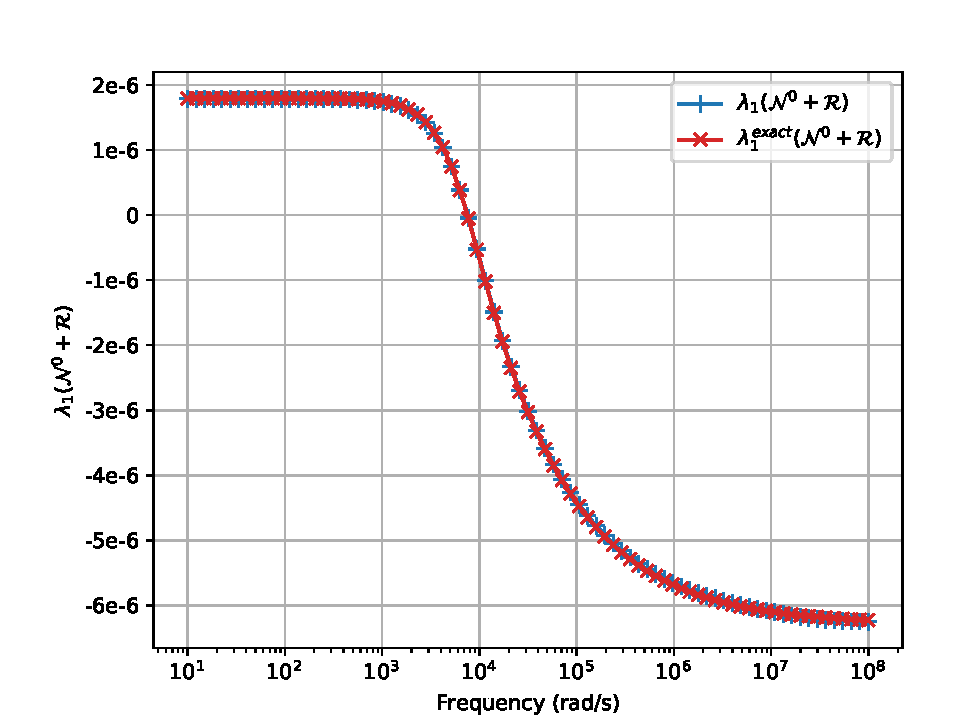
\includegraphics[width=0.48\textwidth, keepaspectratio]{Figures/FullExactReal/FullExactReal.pdf} & 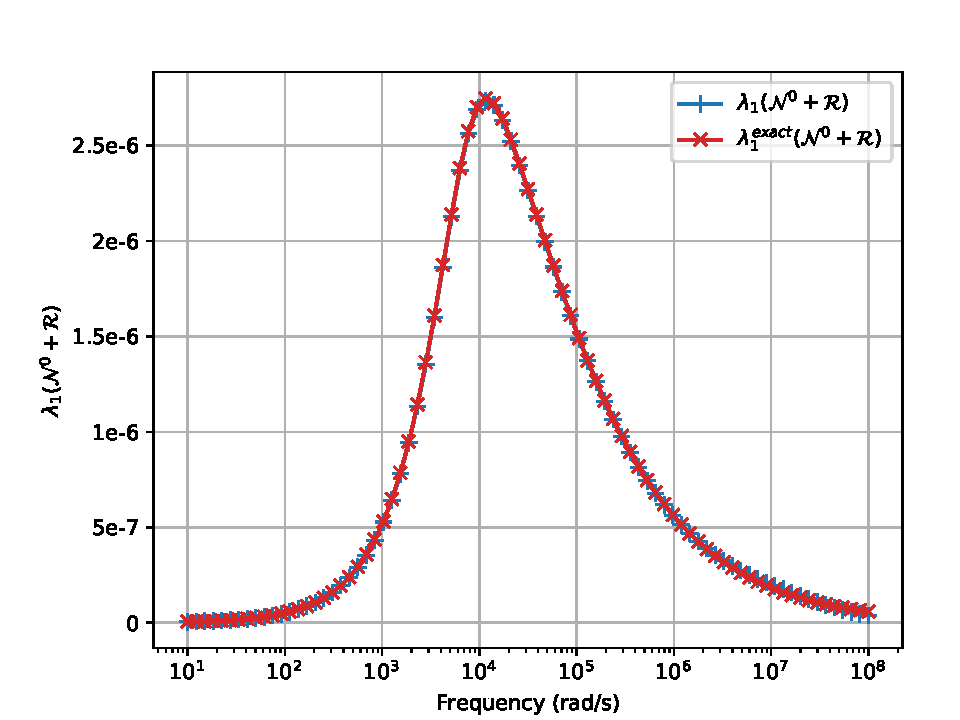
\includegraphics[width=0.48\textwidth, keepaspectratio]{Figures/FullExactImag/FullExactImag.pdf}\\
\textrm{\footnotesize{(a) A graph showing how $\lambda_1(\mathcal{N}^0+\mathcal{R})$ changes with frequency.}} & \textrm{\footnotesize{(b) A graph showing how $\lambda_1(\mathcal{I})$ changes with frequency.}}
\end{array}$$
%\begin{figure}\label{LogvsLin}
\caption{Graphs displaying the eigenvalues of both the real and imaginary parts for $\mathcal{M}$ calculated using a full order frequency sweep for a sphere compared with the exact values.}
\label{fig:FullOrderSphere}
\end{figure}
\noindent
In Figure \ref{fig:FullOrderSphere}, we only show the first eigenvalues $\lambda_1({\mathcal R}+{\mathcal N}^0)$ and $\lambda_1({\mathcal I})$, this is due to the difference between $\lambda_1,\lambda_2,\lambda_3$ being negligible in each case. We also show the exact values of the eigenvalues, which corresponds to the diagonal coefficients of the tensors in this case~\cite{LedgerLionheart2018,Wait1951}, in order to illustrate the performance of the sweep. Note that the code does not produce the exact value for  $\lambda_1({\mathcal R}+{\mathcal N}^0)$ and $\lambda_1({\mathcal I})$ and these have been included afterwards for demonstration purposes. From a visual inspection, the simulation has obtained very good results and this is confirmed by a sweep of  the relative error shown in Figure \ref{fig:FullOrderSphereError}, which shows the maximum relative error is 0.006 over the  sweep.
\begin{figure}[H]
\begin{center}
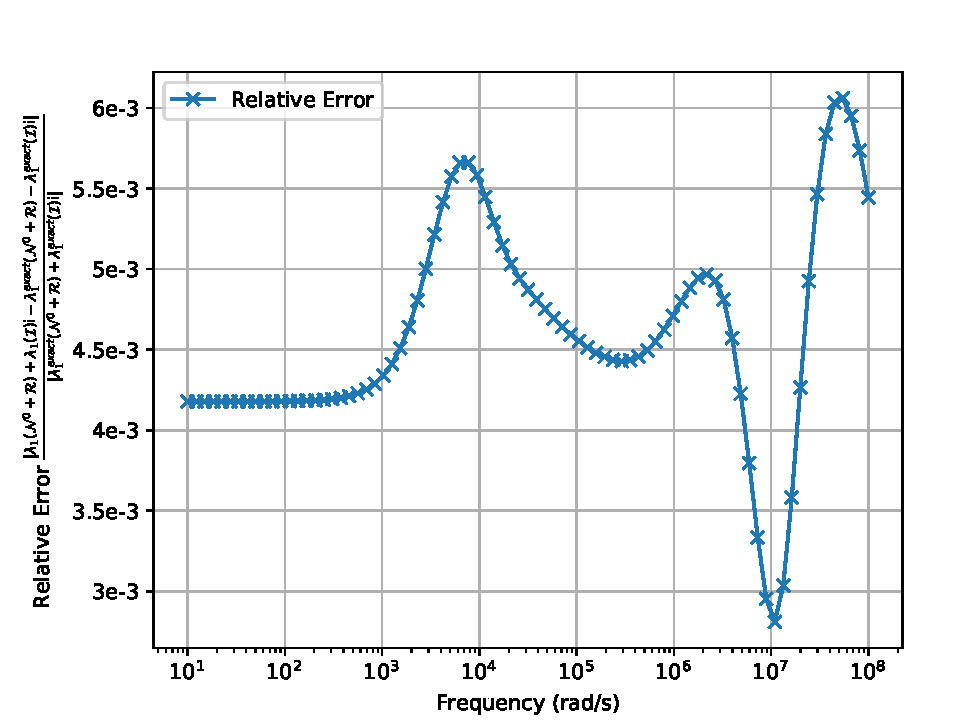
\includegraphics[width=0.5\textwidth]{Figures/FullError/FullError.pdf}
\caption{A graph showing how the relative error in the first eigenvalue changes due to frequency.}\label{fig:FullOrderSphereError}
\end{center}
\end{figure}
\noindent
We next consider the case of a the reduced order frequency sweep using the POD.
\subsubsection{POD frequency sweep for a sphere}
For this frequency sweep , the sphere described by the \texttt{sphere.geo} file in Figure \ref{fig:SweepSphere} is simulated with the inputs as shown in Table \ref{tab:SpherePODInputs}. As  \texttt{Single = False} the following variables are not used:  \texttt{Omega = 133.5}  hence their values are arbitrary.
%\begin{table}[H]
%\begin{center}
%\begin{tabular}{!\vrule l!\vrule l!\vrule l!\vrule}
%\hline
%\texttt{Geometry = "sphere.geo"} & \texttt{Pod = True} & \texttt{EddyCurrentTest = False}\\\hline
%\texttt{alpha = 0.01} & \texttt{MultiProcessing = True} & \texttt{vtk\_output = False}\\\hline
%\texttt{MeshSize = 2} & \texttt{CPUs = 4} & \texttt{Refine\_vtk = False}\\\hline
%\texttt{Order = 3} & \texttt{BigProblem = False} & \texttt{FolderName = "Default"}\\\hline
%\texttt{Start = 1} & \texttt{PODPoints = 13} & \texttt{Solver = "bddc"}\\\hline
%\texttt{Finish = 8} & \texttt{PODTol = 0.0001} & \texttt{epsi = 1e-10}\\\hline
%\texttt{Points = 81} & \texttt{OldMesh = False} & \texttt{Maxsteps = 1500}\\\hline
%\texttt{Single = False} & \texttt{PlotPod = True} & \texttt{Tolerance = 1e-08}\\\hline
%\texttt{Omega = 133.5} & \texttt{PODErrorBars = False} & \texttt{ngsglobals.msg\_level = 0}\\\hline
%\end{tabular}
\begin{table}[H]
\begin{center}
\large{\texttt{main.py}}\normalsize{ }\\\vspace{0.2cm}
\begin{tabular}{!\vrule p{4.5cm}!\vrule p{4.5cm}!\vrule p{4.5cm}!\vrule}
\hline
\texttt{Geometry = "sphere.geo"} & \texttt{alpha = 0.01} & \texttt{MeshSize = 2}\\\hline
\texttt{Order = 3} & \texttt{Start = 1} & \texttt{Finish = 8}\\\hline
\texttt{Points = 81} & \texttt{Single = False} &\texttt{Omega = 133.5}\\\hline
\end{tabular}\\
\begin{tabular}{!\vrule p{4.5cm}!\vrule p{4.5cm}!\vrule}
\texttt{Pod = True} & \texttt{MultiProcessing = True}\\\hline
\end{tabular}
\\\vspace{0.5cm}\large{\texttt{Settings.py}}\normalsize{ }\\\vspace{0.2cm}
\begin{tabular}{!\vrule p{4.5cm}!\vrule p{4.5cm}!\vrule p{4.5cm}!\vrule}
\hline
\texttt{CPUs = 4} & \texttt{BigProblem = False} & \texttt{PODPoints = 13}\\\hline
\texttt{PODTol = 0.0001} & \texttt{OldMesh = False} & \texttt{PlotPod = True}\\\hline
\texttt{PODErrorBars = False} & \texttt{EddyCurrentTest = False} & \texttt{vtk\_output = False}\\\hline
\texttt{Refine\_vtk = False} & \texttt{FolderName = "Default"} & \texttt{Solver = "bddc"}\\\hline
\texttt{epsi = 1e-10} & \texttt{Maxsteps = 1500} & \texttt{Tolerance = 1e-08}\\\hline
\end{tabular}\\
\begin{tabular}{!\vrule p{4.5cm}!\vrule}
\texttt{ngsglobals.msg\_level = 0}\\\hline
\end{tabular}
\caption{A table summarising the inputs for the simulation of a sphere for a reduced order frequency sweep.}\label{tab:SpherePODInputs}
\end{center}
\end{table}
\noindent
This means our interest lies in computing the characterisation for $\alpha B=0.01 B$ at 81 output frequencies in the range $10^1\leq\omega\leq10^8\text{rad/s}$ using  the same mesh of 29170 elements and a $p=3$ discretisation. However, the result is now generated by using a POD technique in which  $13$ snapshots are chosen logarithmically (following the approach described in Section \ref{sectmain.py}) in order to create to create the ROM. On a 2012 iMac with a 2.9 GHz quad core i5 processor with 16 GB 1600 MHz DDR3 memory the computation took 12 minutes and 28 seconds using $4$ CPUs leading to the results shown in Figure \ref{fig:PODSphere}\footnote{The POD frequency sweep in Figure \ref{fig:PODSphere} has been produced with \texttt{ImagTensorFullOrderCalc = True} see Section \ref{Issues} for more details.}.
\begin{figure}[H]
$$\begin{array}{cc}
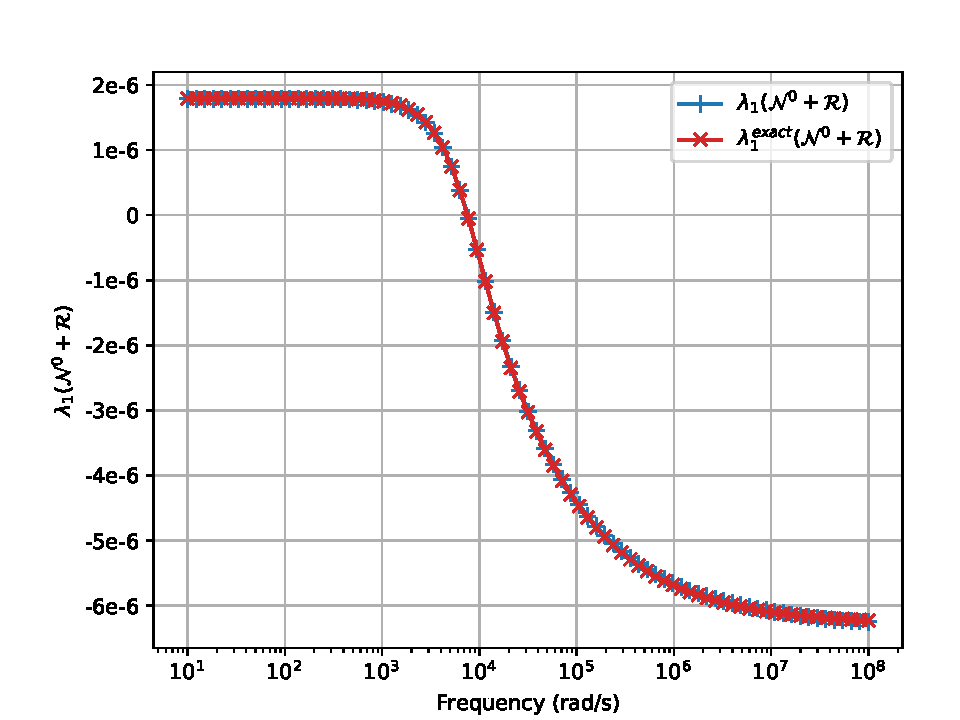
\includegraphics[width=0.48\textwidth, keepaspectratio]{Figures/PODExactReal/PODExactReal.pdf} & 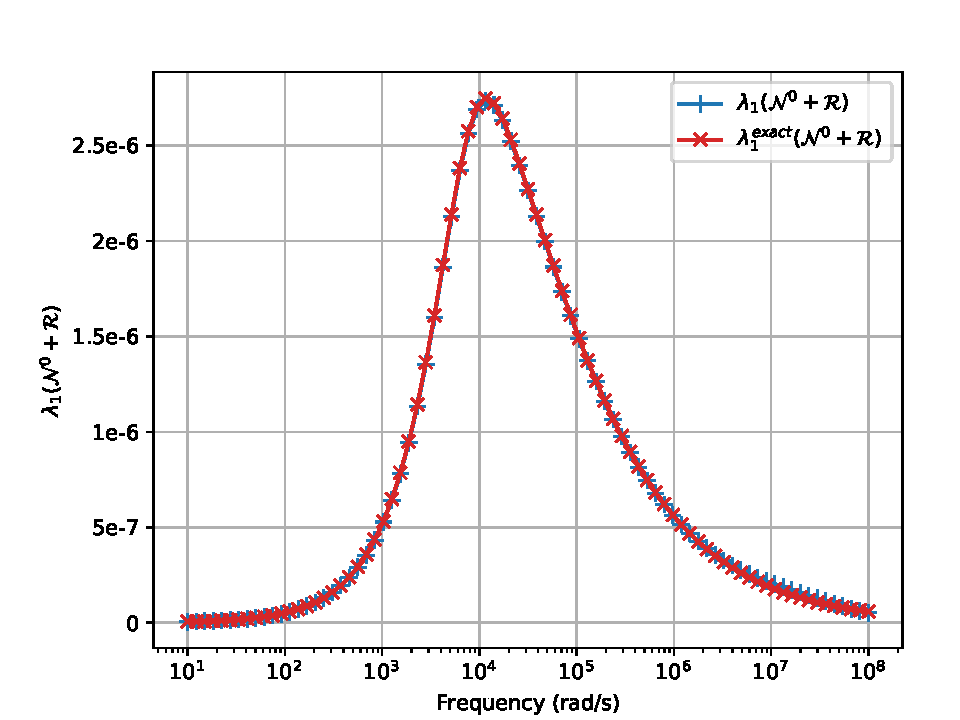
\includegraphics[width=0.48\textwidth, keepaspectratio]{Figures/PODExactImag/PODExactImag.pdf}\\
\textrm{\footnotesize{(a) A graph showing how $\lambda_1(\mathcal{N}^0+\mathcal{R})$ changes with frequency.}} & \textrm{\footnotesize{(b) A graph showing how $\lambda_1(\mathcal{I})$ changes with frequency.}}
\end{array}$$
%\begin{figure}\label{LogvsLin}
\caption{Graphs displaying the eigenvalues of both the real and imaginary parts for $\mathcal{M}$ calculated using a frequency sweep which implemented a POD for a sphere compared with the exact values.}
\label{fig:PODSphere}
\end{figure}
\noindent
Again only the first eigenvalues $\lambda_1({\mathcal R}+{\mathcal N}^0)$ and $\lambda_1({\mathcal I})$ are shown  together with their exact values, added in a post-processing step. From Figure \ref{fig:PODSphere}, we see that the sweep is very accurate and this is confirmed by showing the relative error as a function of frequency  in Figure \ref{fig:PODSphereError}.
\begin{figure}[H]
\begin{center}
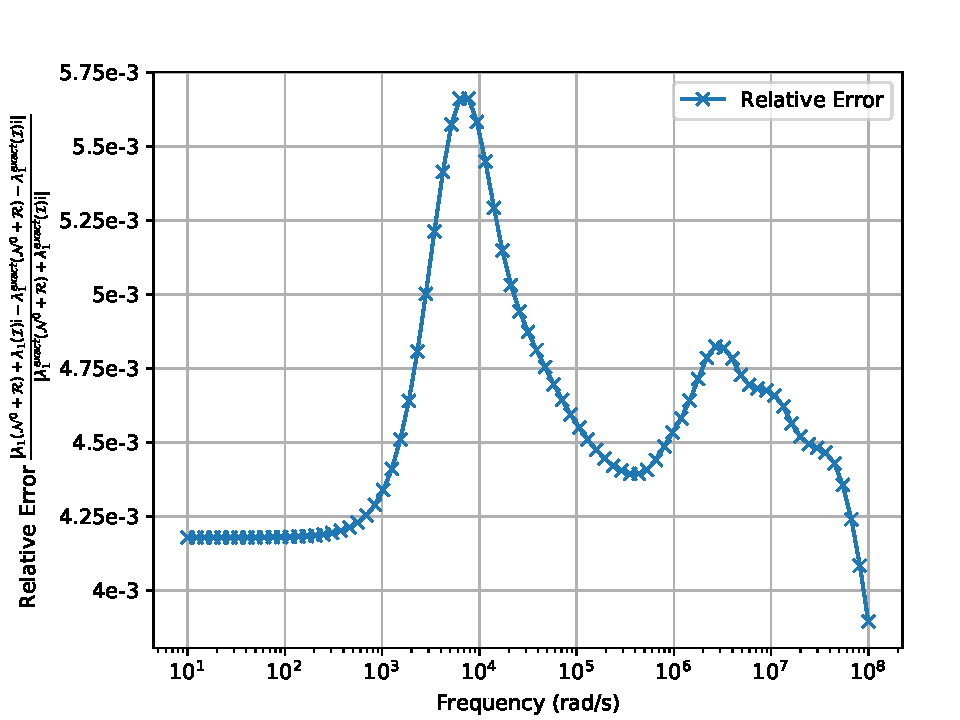
\includegraphics[width=0.5\textwidth]{Figures/PODError/PODError.pdf}
\caption{A graph showing how the relative error in the first eigenvalue changes due to frequency.}\label{fig:PODSphereError}
\end{center}
\end{figure}
\noindent
From Figure \ref{fig:PODSphereError}, we see that the performance is good, if not better, than the full order model, but only requires $13$ full order model snapshots
and took a quarter of the time of the full order model. However, if we set \texttt{PODErrorBars =True} then we obtain upper bounds on the difference between the full order and POD frequency sweeps. An example of this can be seen in Figure \ref{fig:PODSphereErrorBars} this was run for 21 snapshots with a POD tolerance of $10^{-6}$. Note that these certificate bounds are computed at run time with minimal additional computational cost. For further details of the cost break down and additional examples of certificate bounds see \cite{wilsonledger2019}.
\begin{figure}[H]
$$\begin{array}{cc}
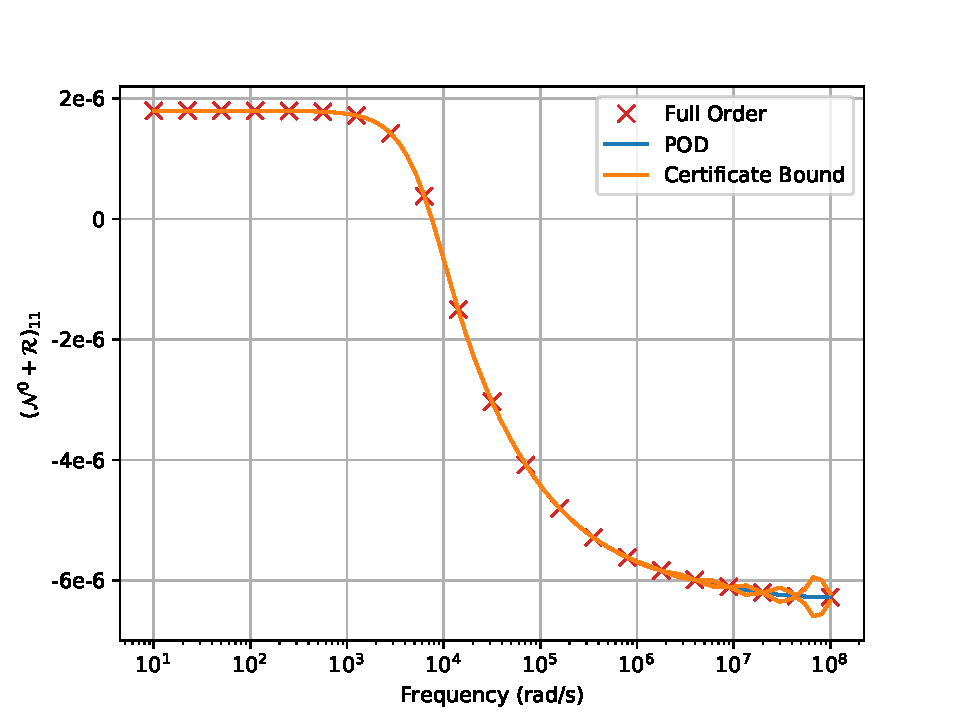
\includegraphics[width=0.48\textwidth, keepaspectratio]{Figures/SphereErrorBarsRealn=21.pdf} & 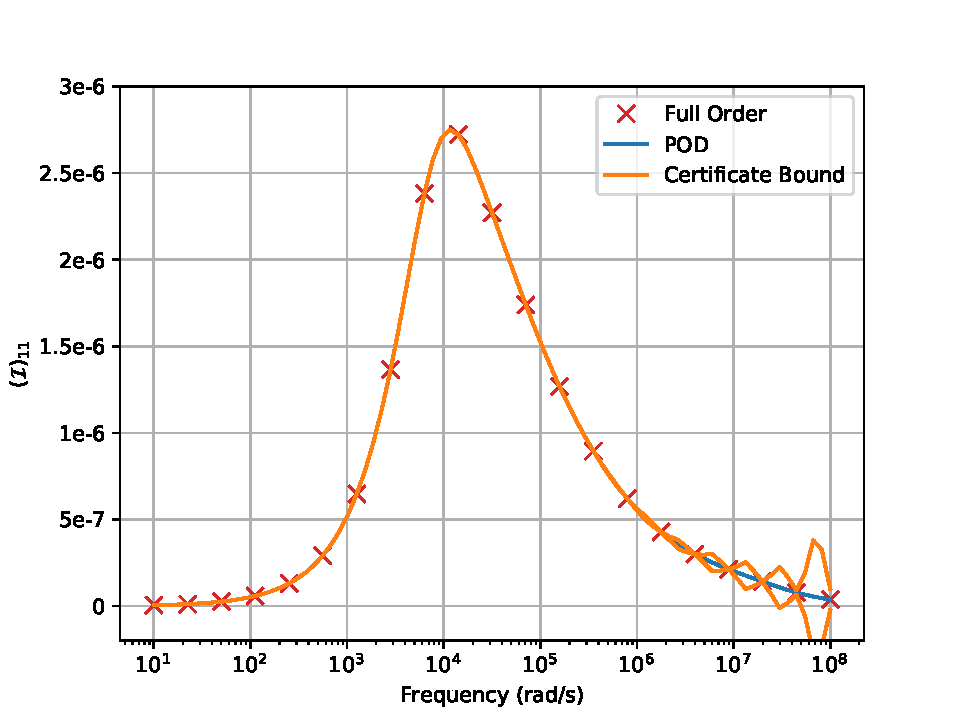
\includegraphics[width=0.48\textwidth, keepaspectratio]{Figures/SphereErrorBarsImagn=21.pdf}\\
\textrm{\footnotesize{(a) A graph showing how $(\mathcal{N}^0+\mathcal{R})_{11}$ changes with frequency.}} & \textrm{\footnotesize{(b) A graph showing how $(\mathcal{I})_{11}$ changes with frequency.}}
\end{array}$$
\caption{A graph showing the certificate bounds produced for the sphere with 21 snapshots with a POD tolerance of $10^{-6}$.}\label{fig:PODSphereErrorBars}
\end{figure}
\noindent
For more detail about how the bounds are computed along with other examples please see \cite{wilsonledger2019}. With this we conclude the examples of the sphere, we next consider a simulation of a conducting permeable torus.
\subsection{Torus}
In this section, we consider the case where $B$  is a torus with a major and minor radii of  of 2 and  1, respectively, and the physical object $\alpha B$ is created from this object using the scaling $\alpha=0.01\text{m}$. We simulate a full order frequency sweep using the \texttt{Torus.geo} file shown in Figure \ref{fig:torus.geo}, where $\Omega$ is chosen to be a ball of radius 100 containing the object $B$ with material parameters $\sigma_*=5.96\times10^6\text{ S/m}$ and $\mu_*=1.5\mu_0$.
\begin{figure}[H]
\begin{center}
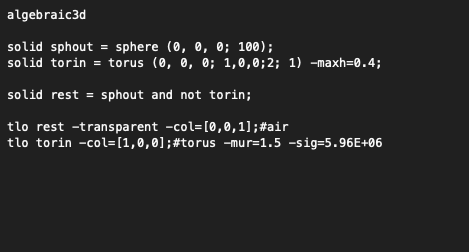
\includegraphics[width=0.5\textwidth]{Figures/TorusInput.png}
\caption{An image showing the \texttt{Torus.geo} file used to simulate the torus.}\label{fig:torus.geo}
\end{center}
\end{figure}
\noindent
To set up this simulation, we used the \texttt{Torus.geo} file shown in Figure \ref{fig:torus.geo} along with the inputs summarised in Table \ref{tab:TorusInputs}.
%\begin{table}[H]
%\begin{center}
%\begin{tabular}{!\vrule l!\vrule l!\vrule l!\vrule}
%\hline
%\texttt{Geometry = "Torus.geo"} & \texttt{Pod = False} & \texttt{EddyCurrentTest = False}\\\hline
%\texttt{alpha = 0.01} & \texttt{MultiProcessing = True} & \texttt{vtk\_output = False}\\\hline
%\texttt{MeshSize = 3} & \texttt{CPUs = 4} & \texttt{Refine\_vtk = False}\\\hline
%\texttt{Order = 3} & \texttt{BigProblem = False} & \texttt{FolderName = "Default"}\\\hline
%\texttt{Start = 1} & \texttt{PODPoints = 13} & \texttt{Solver = "bddc"}\\\hline
%\texttt{Finish = 8} & \texttt{PODTol = 0.0001} & \texttt{epsi = 1e-10}\\\hline
%\texttt{Points = 81} & \texttt{OldMesh = False} & \texttt{Maxsteps = 1500}\\\hline
%\texttt{Single = False} & \texttt{PlotPod = True} & \texttt{Tolerance = 1e-08}\\\hline
%\texttt{Omega = 133.5} & \texttt{PODErrorBars = False} & \texttt{ngsglobals.msg\_level = 0}\\\hline
%\end{tabular}
\begin{table}[H]
\begin{center}
\large{\texttt{main.py}}\normalsize{ }\\\vspace{0.2cm}
\begin{tabular}{!\vrule p{4.5cm}!\vrule p{4.5cm}!\vrule p{4.5cm}!\vrule}
\hline
\texttt{Geometry = "Torus.geo"} & \texttt{alpha = 0.01} & \texttt{MeshSize = 3}\\\hline
\texttt{Order = 3} & \texttt{Start = 1} & \texttt{Finish = 8}\\\hline
\texttt{Points = 81} & \texttt{Single = False} &\texttt{Omega = 133.5}\\\hline
\end{tabular}\\
\begin{tabular}{!\vrule p{4.5cm}!\vrule p{4.5cm}!\vrule}
\texttt{Pod = False} & \texttt{MultiProcessing = True}\\\hline
\end{tabular}
\\\vspace{0.5cm}\large{\texttt{Settings.py}}\normalsize{ }\\\vspace{0.2cm}
\begin{tabular}{!\vrule p{4.5cm}!\vrule p{4.5cm}!\vrule p{4.5cm}!\vrule}
\hline
\texttt{CPUs = 4} & \texttt{BigProblem = False} & \texttt{PODPoints = 13}\\\hline
\texttt{PODTol = 0.0001} & \texttt{OldMesh = False} & \texttt{PlotPod = True}\\\hline
\texttt{PODErrorBars = False} & \texttt{EddyCurrentTest = False} & \texttt{vtk\_output = False}\\\hline
\texttt{Refine\_vtk = False} & \texttt{FolderName = "Default"} & \texttt{Solver = "bddc"}\\\hline
\texttt{epsi = 1e-10} & \texttt{Maxsteps = 1500} & \texttt{Tolerance = 1e-08}\\\hline
\end{tabular}\\
\begin{tabular}{!\vrule p{4.5cm}!\vrule}
\texttt{ngsglobals.msg\_level = 0}\\\hline
\end{tabular}
\caption{A table summarising the inputs for the simulation of a torus for a reduced order frequency sweep.}
\label{tab:TorusInputs}
\end{center}
\end{table}
\noindent
This means our interest lies in computing the characterisation for $\alpha B=0.01B$ at 81 frequencies in the range $10^1\leq\omega\leq10^8\text{ rad/s}$. Furthermore, the inputs lead to a mesh of 32008 elements and a discretisation of $p=3$. On a 2012 iMac with a 2.9 GHz quad core i5 processor with 16 GB 1600 MHz DDR3 memory the computation takes 57 minutes 15 seconds using 4 CPUs (POD offers a considerable savings and comparable accuracy, see below). Using \texttt{Order = 0} and the above settings has a run time of only 22 minutes 57 seconds, but with lower accuracy. In this case, the inputs in \texttt{PlotterSettings.py} are chosen to be as summarised in Table \ref{tab:TorusPlotterInputs}\footnote{We chosen to not list the \texttt{Show} variable as this determines whether the graphs are show at the time of making.}, which leads to the results shown in Figure \ref{fig:TorusOutput}.
\begin{table}[H]
\begin{center}
\begin{tabular}{!\vrule l!\vrule l!\vrule}
\hline
\texttt{EigsToPlot = [1,2,3]}  & \texttt{TensorsToPlot = [1,4,6,2,3,5]} \\\hline
\texttt{MainLineStyle = "-"} & \texttt{MainMarkerSize = 4} \\\hline
\texttt{SnapshotLineStyle = "x"} & \texttt{SnapshotMarkerSize = 8} \\\hline
\texttt{ErrorBarLineStyle = "--"} & \texttt{ErrorBarMarkerSize = 4} \\\hline
\texttt{Title = True} &  \texttt{EddyCurrentLine = False}\\\hline
\end{tabular}
\caption{A table summarising the inputs for the plots produced by the simulation of a torus using a reduced order frequency sweep.}
\label{tab:TorusPlotterInputs}
\end{center}
\end{table}
\begin{figure}[H]
$$\begin{array}{cc}
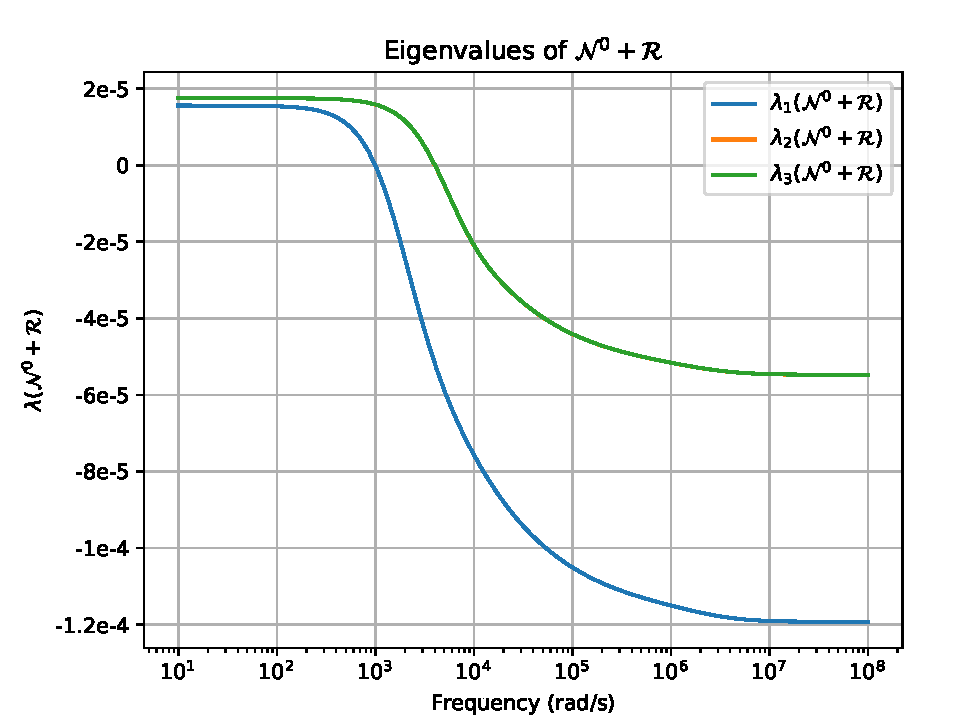
\includegraphics[width=0.48\textwidth, keepaspectratio]{Figures/Torus/RealEigenvalues.pdf} & 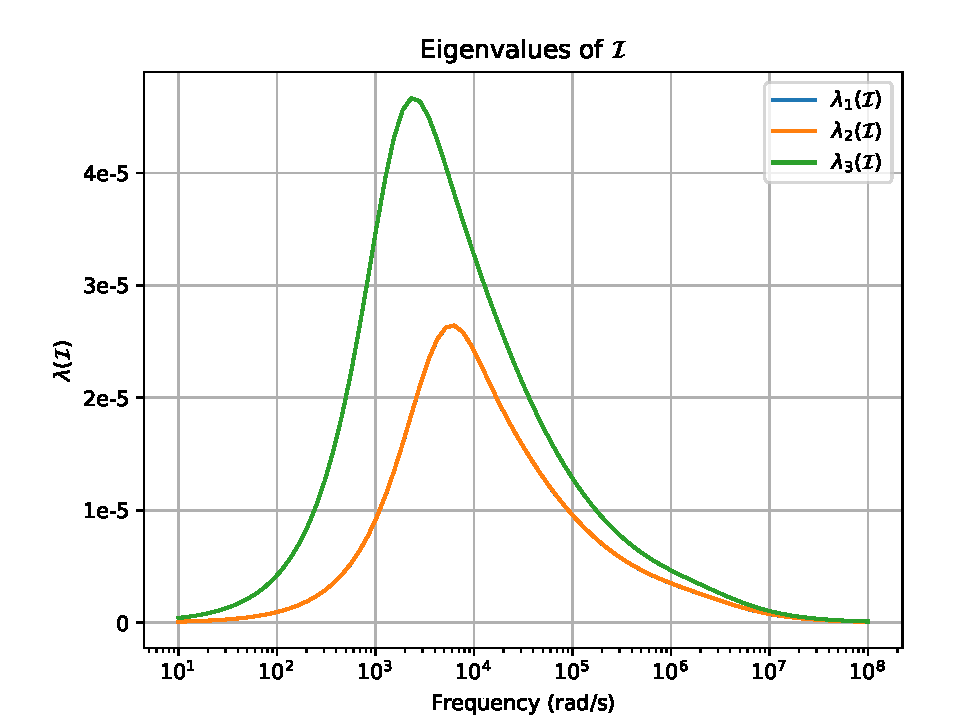
\includegraphics[width=0.48\textwidth, keepaspectratio]{Figures/Torus/ImaginaryEigenvalues.pdf}\\
\textrm{\footnotesize{(a) A graph showing how $\lambda_i(\mathcal{N}^0+\mathcal{R})$ changes with frequency.}} & \textrm{\footnotesize{(b) A graph showing how $\lambda_i(\mathcal{I})$ changes with frequency.}}\\
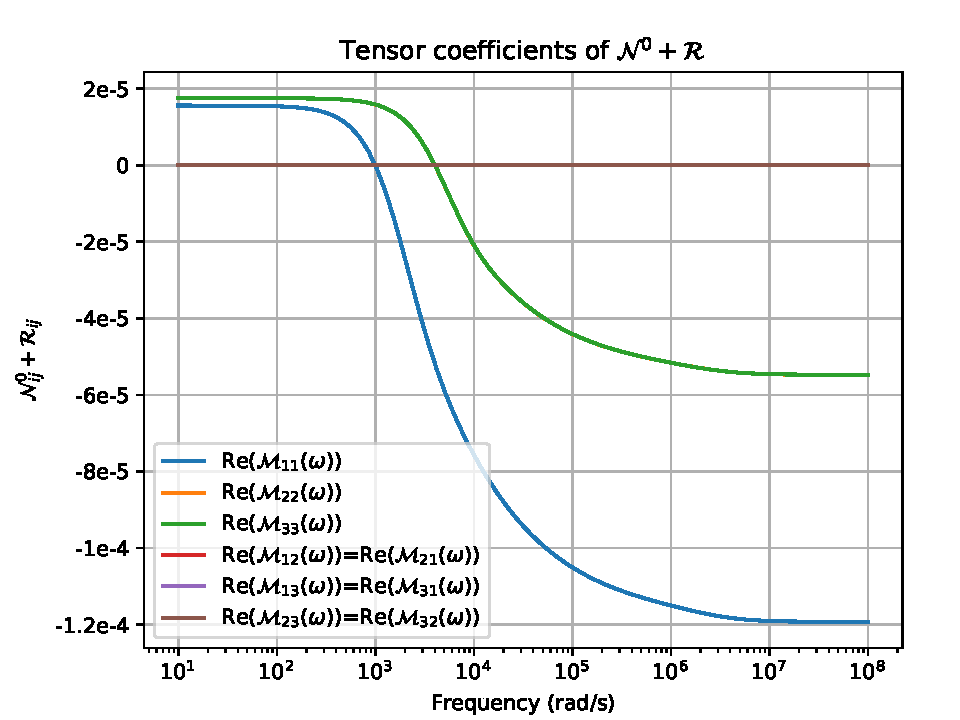
\includegraphics[width=0.48\textwidth, keepaspectratio]{Figures/Torus/RealTensorCoeficients.pdf} & 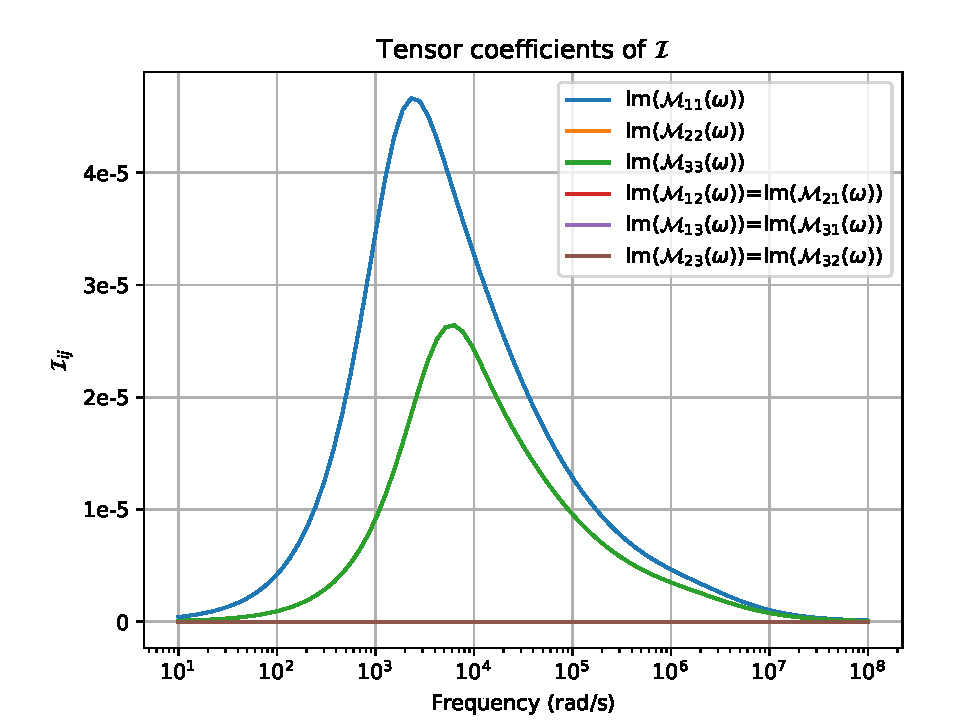
\includegraphics[width=0.48\textwidth, keepaspectratio]{Figures/Torus/ImaginaryTensorCoeficients.pdf}\\
\textrm{\footnotesize{(c) A graph showing how $\mathcal{N}^0_{ij}+\mathcal{R}_{ij}$ change with frequency.}} & \textrm{\footnotesize{(d) A graph showing how $\mathcal{I}_{ij}$ change with frequency.}}
\end{array}$$
%\begin{figure}\label{LogvsLin}
\caption{Graphs displaying the eigenvalues and tensor coefficients of both the real and imaginary parts for $\mathcal{M}$ calculated using a full order frequency sweep for a torus.}
\label{fig:TorusOutput}
\end{figure}
\noindent
This means that the eigenvalues $\lambda_i(\mathcal{N}^0+\mathcal{R})$, $\lambda_i(\mathcal{I})$, $i=1,2,3$ are computed and shown as a function of frequency along with tensor coefficients $\mathcal{N}^0_{ij}+\mathcal{R}_{ij}$, $\mathcal{I}_{ij}$ for the combinations $(i,j) =\{ (1,1), (2,2), (3,3),(1,2)=(2,1), (1,3)=(3,1), (2,3)=(3,2)\}$. We note that the object has rotational and reflectional symmetries and so it has only $2$ independent coefficients corresponding to tensor indices  
$(1,1)$ and $(2,2)=(3,3)$~\cite{LedgerLionheart2015,LedgerLionheart2016}. 

Repeating the same simulation with  \texttt{Pod = True} in Table~\ref{tab:TorusInputs} results in similar results, but only takes 14 minutes 38 seconds, which is a substantial saving. 


With this we conclude our example of the torus, we next consider the example of a tetrahedron.


\subsection{Tetrahedron}
In this section, we consider the case where $B$ is an irregular tetrahedron with vertices 
\begin{equation}
(0,0,0),  \qquad (7,0,0), \qquad  (5.5, 4.6,0), \qquad (3.3, 2.0, 0.5)
\nonumber
\end{equation}
and $\alpha B$ is the irregular tetrahedron produced using the scaling $\alpha=0.01\text{m}$.

The geometry is described by  \texttt{Tetra.geo} file as shown in Figure \ref{fig:Tetra.geo}, where $\Omega$ is chosen to be a cube with sides of length 200 containing the object $B$ and its material parameters are $\sigma_*=5.96\times10^6\text{ S/m}$ and $\mu_*=2\mu_0$.
\begin{figure}[H]
\begin{center}
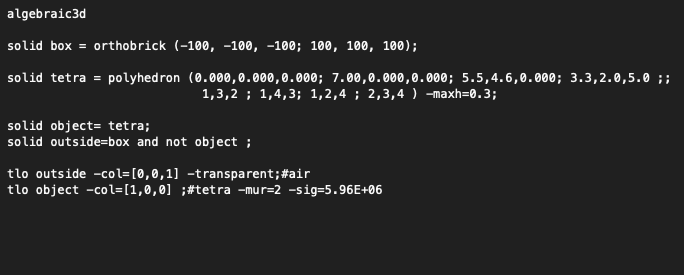
\includegraphics[width=0.7\textwidth]{Figures/TetraInput.png}
\caption{An image showing the \texttt{Tetra.geo} file used to simulate the torus.}\label{fig:Tetra.geo}
\end{center}
\end{figure}
\noindent
The inputs for this simulation are summarised in Table \ref{tab:TetraInputs}.
%\begin{table}[H]
%\begin{center}
%\begin{tabular}{!\vrule l!\vrule l!\vrule l!\vrule}
%\hline
%\texttt{Geometry = "Tetra.geo"} & \texttt{Pod = True} & \texttt{EddyCurrentTest = False}\\\hline
%\texttt{alpha = 0.01} & \texttt{MultiProcessing = True} & \texttt{vtk\_output = False}\\\hline
%\texttt{MeshSize = 3} & \texttt{CPUs = 4} & \texttt{Refine\_vtk = False}\\\hline
%\texttt{Order = 3} & \texttt{BigProblem = False} & \texttt{FolderName = "Default"}\\\hline
%\texttt{Start = 2} & \texttt{PODPoints = 13} & \texttt{Solver = "bddc"}\\\hline
%\texttt{Finish = 8} & \texttt{PODTol = 0.0001} & \texttt{epsi = 1e-10}\\\hline
%\texttt{Points = 81} & \texttt{OldMesh = False} & \texttt{Maxsteps = 1500}\\\hline
%\texttt{Single = False} & \texttt{PlotPod = True} & \texttt{Tolerance = 1e-08}\\\hline
%\texttt{Omega = 133.5} & \texttt{PODErrorBars = False} & \texttt{ngsglobals.msg\_level = 0}\\\hline
%\end{tabular}
\begin{table}[H]
\begin{center}
\large{\texttt{main.py}}\normalsize{ }\\\vspace{0.2cm}
\begin{tabular}{!\vrule p{4.5cm}!\vrule p{4.5cm}!\vrule p{4.5cm}!\vrule}
\hline
\texttt{Geometry = "Tetra.geo"} & \texttt{alpha = 0.01} & \texttt{MeshSize = 3}\\\hline
\texttt{Order = 3} & \texttt{Start = 2} & \texttt{Finish = 8}\\\hline
\texttt{Points = 81} & \texttt{Single = False} &\texttt{Omega = 133.5}\\\hline
\end{tabular}\\
\begin{tabular}{!\vrule p{4.5cm}!\vrule p{4.5cm}!\vrule}
\texttt{Pod = True} & \texttt{MultiProcessing = True}\\\hline
\end{tabular}
\\\vspace{0.5cm}\large{\texttt{Settings.py}}\normalsize{ }\\\vspace{0.2cm}
\begin{tabular}{!\vrule p{4.5cm}!\vrule p{4.5cm}!\vrule p{4.5cm}!\vrule}
\hline
\texttt{CPUs = 4} & \texttt{BigProblem = False} & \texttt{PODPoints = 13}\\\hline
\texttt{PODTol = 0.0001} & \texttt{OldMesh = False} & \texttt{PlotPod = True}\\\hline
\texttt{PODErrorBars = False} & \texttt{EddyCurrentTest = False} & \texttt{vtk\_output = False}\\\hline
\texttt{Refine\_vtk = False} & \texttt{FolderName = "Default"} & \texttt{Solver = "bddc"}\\\hline
\texttt{epsi = 1e-10} & \texttt{Maxsteps = 1500} & \texttt{Tolerance = 1e-08}\\\hline
\end{tabular}\\
\begin{tabular}{!\vrule p{4.5cm}!\vrule}
\texttt{ngsglobals.msg\_level = 0}\\\hline
\end{tabular}
\caption{A table summarising the inputs for the simulation of an irregular tetrahedron for a reduced order frequency sweep.}\label{tab:TetraInputs}
\end{center}
\end{table}
\noindent
This means our interest lies in computing the characterisation for $\alpha B=0.01B$ at 81 frequencies in the range $10^1\leq\omega\leq10^8\text{ rad/s}$. Furthermore, the inputs lead to a mesh of 22923 elements and a discretisation of $p=3$.  In this case, a POD technique using  $13$ snapshots chosen logarithmically (following the approach described in Section \ref{sectmain.py}) is used  to create to create the ROM. On a 2012 iMac with a 2.9 GHz quad core i5 processor with 16 GB 1600 MHz DDR3 memory the computation takes 7 minutes and 18 seconds using 4 CPUs. 

The inputs in \texttt{PlotterSettings.py} are summarised in Table \ref{tab:TetraPlotterInputs} leading to the results shown  in Figure \ref{fig:TetraOutputs}.
\begin{table}[H]
\begin{center}
\begin{tabular}{!\vrule l!\vrule l!\vrule}
\hline
\texttt{EigsToPlot = [1,2,3]}  & \texttt{TensorsToPlot = [1,4,6,2,3,5]} \\\hline
\texttt{MainLineStyle = "-"} & \texttt{MainMarkerSize = 4} \\\hline
\texttt{SnapshotLineStyle = "x"} & \texttt{SnapshotMarkerSize = 8} \\\hline
\texttt{ErrorBarLineStyle = "--"} & \texttt{ErrorBarMarkerSize = 4} \\\hline
\texttt{Title = True} &  \texttt{EddyCurrentLine = False}\\\hline
\end{tabular}
\caption{A table summarising the inputs for the plots produced by the simulation of an irregular tetrahedron using a reduced order frequency sweep.}\label{tab:TetraPlotterInputs}
\end{center}
\end{table}
\begin{figure}[H]
$$\begin{array}{cc}
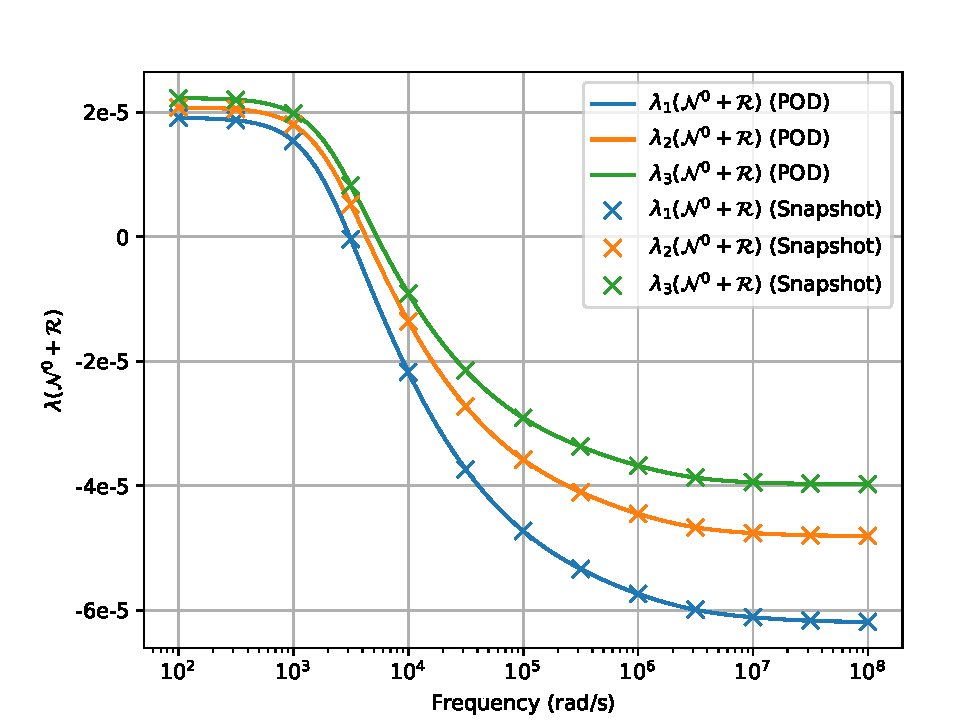
\includegraphics[width=0.48\textwidth, keepaspectratio]{Figures/Tetra/RealEigenvalues.pdf} & 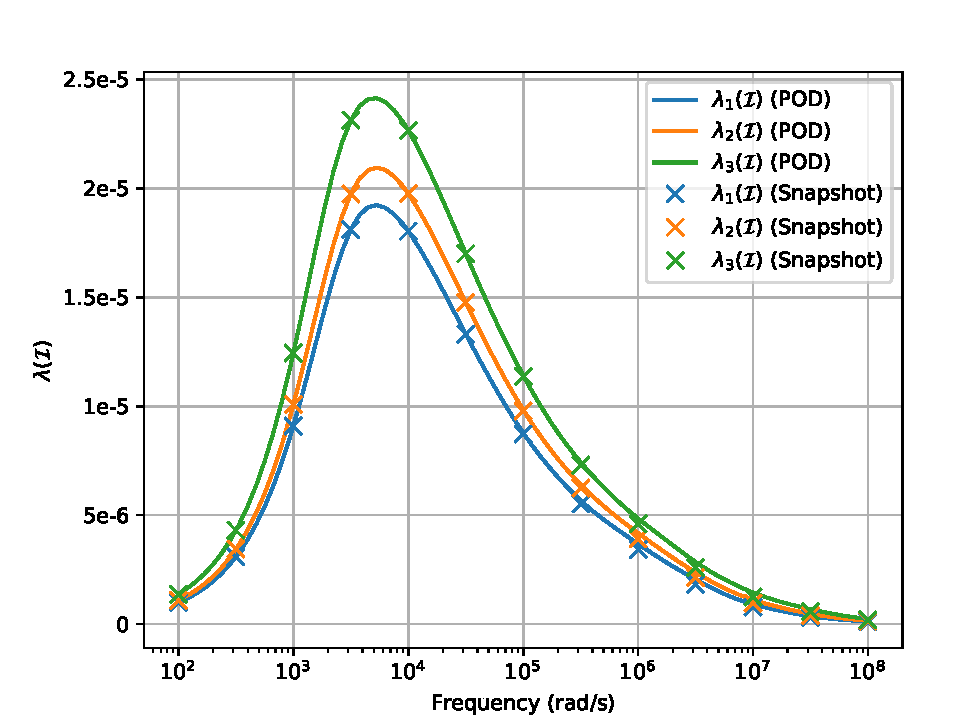
\includegraphics[width=0.48\textwidth, keepaspectratio]{Figures/Tetra/ImaginaryEigenvalues.pdf}\\
\textrm{\footnotesize{(a) A graph showing how $\lambda(\mathcal{N}^0+\mathcal{R})$ changes with frequency.}} & \textrm{\footnotesize{(b) A graph showing how $\lambda(\mathcal{I})$ changes with frequency.}}\\
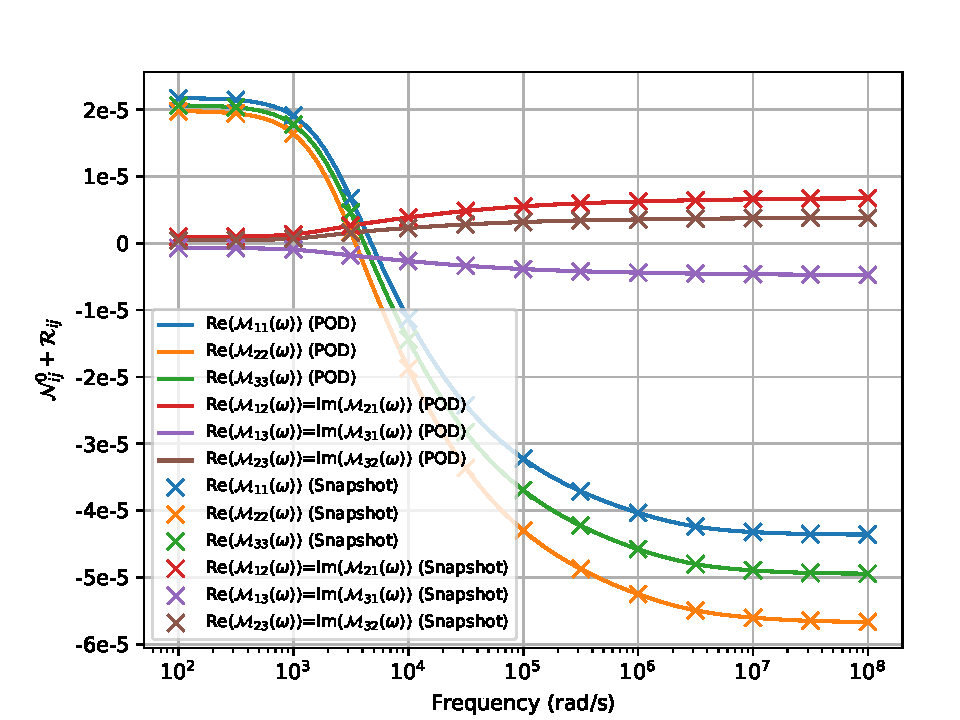
\includegraphics[width=0.48\textwidth, keepaspectratio]{Figures/Tetra/RealTensorCoeficients.pdf} & 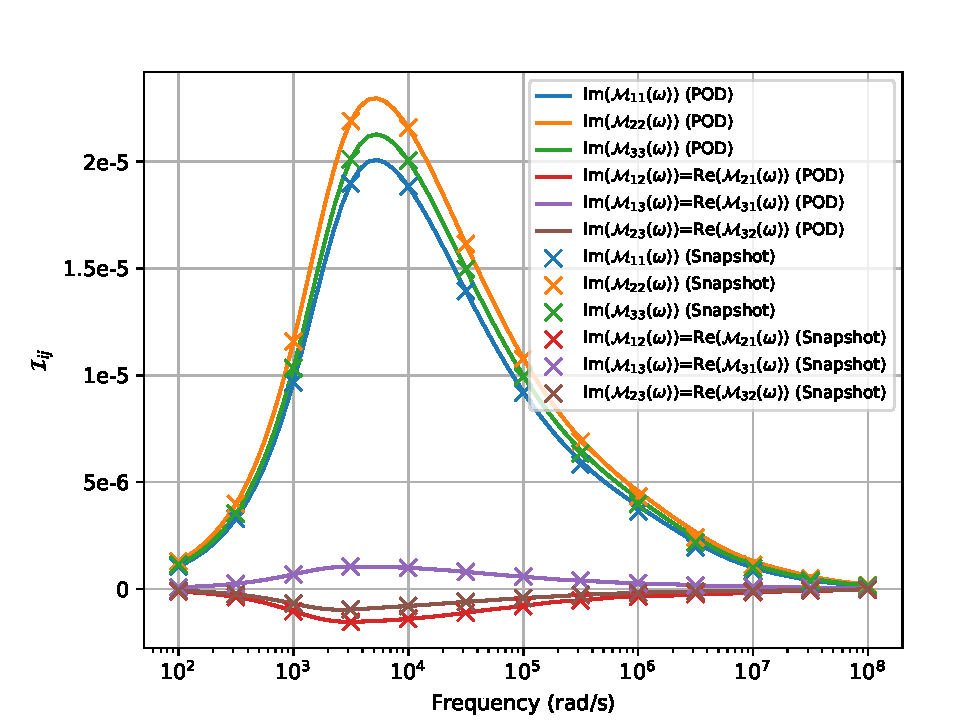
\includegraphics[width=0.48\textwidth, keepaspectratio]{Figures/Tetra/ImaginaryTensorCoeficients.pdf}\\
\textrm{\footnotesize{(c) A graph showing how $\mathcal{N}^0_{ij}+\mathcal{R}_{ij}$ change with frequency.}} & \textrm{\footnotesize{(d) A graph showing how $\mathcal{I}_{ij}$ change with frequency.}}
\end{array}$$
%\begin{figure}\label{LogvsLin}
\caption{Graphs displaying the eigenvalues and tensor coefficients of both the real and imaginary parts for $\mathcal{M}$ calculated using a reduced order frequency sweep for a tetrahedron.}
\label{fig:TetraOutputs}
\end{figure}
\noindent
From Figure \ref{fig:TetraOutputs},  we see that $\mathcal{M}$ has 6 independent non-zero coefficients, due to the lack of rotational and reflectional symmetries in the (irregular) tetrahedron. With this we conclude our example of the tetrahedron, we next consider the case of a bar created using two regions.
\subsection{Dual Bar}
In this section we consider $B =B^{(1)} \cup B^{(2)}$  to be a bar created by joining two  rectangular blocks with different parameters. The physical object $\alpha B$ is obtained by scaling $B$ by $\alpha=0.01\text{m}$. The geometry described by the \texttt{DualBar.geo} file in Figure \ref{fig:DualBar.geo}, where $\Omega$ is chosen to be a ball of radius 100 containing the object $B$. Following the notation in~\cite{LedgerLionheartamad2019}, the material parameters of $B^{(1)}$ and $ B^{(2)}$  are
\begin{align*}
\begin{array}{l}
\sigma_*^{(1)}= 10^6\text{ S/m} \\
\sigma_*^{(2)}=10^8\text{ S/m}
\end{array} \qquad  \text{ and } \qquad
\begin{array}{l}
\mu_* ^{(1)}=
\mu_0\\
\mu_* ^{(2)}=\mu_0
\end{array}
\end{align*}
\begin{figure}[H]
\begin{center}
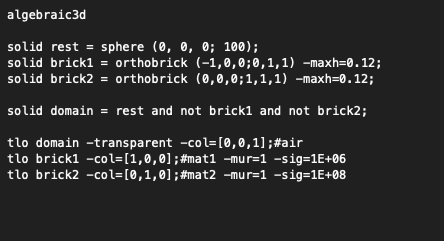
\includegraphics[width=0.6\textwidth]{Figures/DualBarInput.png}
\caption{An image showing the \texttt{DualBar.geo} file used to simulate the torus.}\label{fig:DualBar.geo}
\end{center}
\end{figure}
\noindent


To set up this simulation, we used the \texttt{Dualbar.geo} file shown in Figure \ref{fig:DualBar.geo} along with the inputs summarised in Table \ref{tab:DualBarInputs}
%\begin{table}[H]
%\begin{center}
%\begin{tabular}{!\vrule l!\vrule l!\vrule l!\vrule}
%\hline
%\texttt{Geometry = "DualBar.geo"} & \texttt{Pod = True} & \texttt{EddyCurrentTest = False}\\\hline
%\texttt{alpha = 0.01} & \texttt{MultiProcessing = True} & \texttt{vtk\_output = False}\\\hline
%\texttt{MeshSize = 3} & \texttt{CPUs = 4} & \texttt{Refine\_vtk = False}\\\hline
%\texttt{Order = 3} & \texttt{BigProblem = False} & \texttt{FolderName = "Default"}\\\hline
%\texttt{Start = 2} & \texttt{PODPoints = 9} & \texttt{Solver = "bddc"}\\\hline
%\texttt{Finish = 7} & \texttt{PODTol = 1e-05} & \texttt{epsi = 1e-10}\\\hline
%\texttt{Points = 81} & \texttt{OldMesh = False} & \texttt{Maxsteps = 1500}\\\hline
%\texttt{Single = False} & \texttt{PlotPod = True} & \texttt{Tolerance = 1e-08}\\\hline
%\texttt{Omega = 133.5} & \texttt{PODErrorBars = False} & \texttt{ngsglobals.msg\_level = 0}\\\hline
%\end{tabular}
\begin{table}[H]
\begin{center}
\large{\texttt{main.py}}\normalsize{ }\\\vspace{0.2cm}
\begin{tabular}{!\vrule p{4.5cm}!\vrule p{4.5cm}!\vrule p{4.5cm}!\vrule}
\hline
\texttt{Geometry = "DualBar.geo"} & \texttt{alpha = 0.01} & \texttt{MeshSize = 3}\\\hline
\texttt{Order = 3} & \texttt{Start = 2} & \texttt{Finish = 7}\\\hline
\texttt{Points = 81} & \texttt{Single = False} &\texttt{Omega = 133.5}\\\hline
\end{tabular}\\
\begin{tabular}{!\vrule p{4.5cm}!\vrule p{4.5cm}!\vrule}
\texttt{Pod = True} & \texttt{MultiProcessing = True}\\\hline
\end{tabular}
\\\vspace{0.5cm}\large{\texttt{Settings.py}}\normalsize{ }\\\vspace{0.2cm}
\begin{tabular}{!\vrule p{4.5cm}!\vrule p{4.5cm}!\vrule p{4.5cm}!\vrule}
\hline
\texttt{CPUs = 4} & \texttt{BigProblem = False} & \texttt{PODPoints = 9}\\\hline
\texttt{PODTol = 1e-05} & \texttt{OldMesh = False} & \texttt{PlotPod = True}\\\hline
\texttt{PODErrorBars = False} & \texttt{EddyCurrentTest = False} & \texttt{vtk\_output = False}\\\hline
\texttt{Refine\_vtk = False} & \texttt{FolderName = "Default"} & \texttt{Solver = "bddc"}\\\hline
\texttt{epsi = 1e-10} & \texttt{Maxsteps = 1500} & \texttt{Tolerance = 1e-08}\\\hline
\end{tabular}\\
\begin{tabular}{!\vrule p{4.5cm}!\vrule}
\texttt{ngsglobals.msg\_level = 0}\\\hline
\end{tabular}
\caption{A table summarising the inputs for the simulation of a bar containing two regions for a reduced order frequency sweep.}
\label{tab:DualBarInputs}
\end{center}
\end{table}
\noindent
This means our interest lies in computing the characterisation for $\alpha B=0.01B$ at 81 frequencies in the range $10^2\leq\omega\leq10^7 \text{ rad/s}$. Furthermore, the inputs lead to a mesh of 36772 elements and a discretisation of $p=3$. In this case, a POD technique using  $9$ snapshots chosen logarithmically (following the approach described in Section \ref{sectmain.py}) is used  to create to create the ROM. 
 On a 2012 iMac with a 2.9 GHz quad core i5 processor with 16 GB 1600 MHz DDR3 memory the computation takes 8 minutes and 32 seconds using 4 CPUs. The inputs of \texttt{PLotterSettings.py} are summarised in Table \ref{tab:DualBarPlotterInputs} leading to the results shown in Figure \ref{fig:DualBarOutputs}.
\begin{table}[H]
\begin{center}
\begin{tabular}{!\vrule l!\vrule l!\vrule}
\hline
\texttt{EigsToPlot = [1,2,3]}  & \texttt{TensorsToPlot = [1,4,6]} \\\hline
\texttt{MainLineStyle = "-"} & \texttt{MainMarkerSize = 4} \\\hline
\texttt{SnapshotLineStyle = "o"} & \texttt{SnapshotMarkerSize = 6} \\\hline
\texttt{ErrorBarLineStyle = "--"} & \texttt{ErrorBarMarkerSize = 4} \\\hline
\texttt{Title = False} &  \texttt{EddyCurrentLine = True}\\\hline
\end{tabular}
\caption{A table summarising the inputs for the plots produced by the simulation of bar created using two regions using a reduced order frequency sweep.}\label{tab:DualBarPlotterInputs}
\end{center}
\end{table}
\begin{figure}[H]
$$\begin{array}{cc}
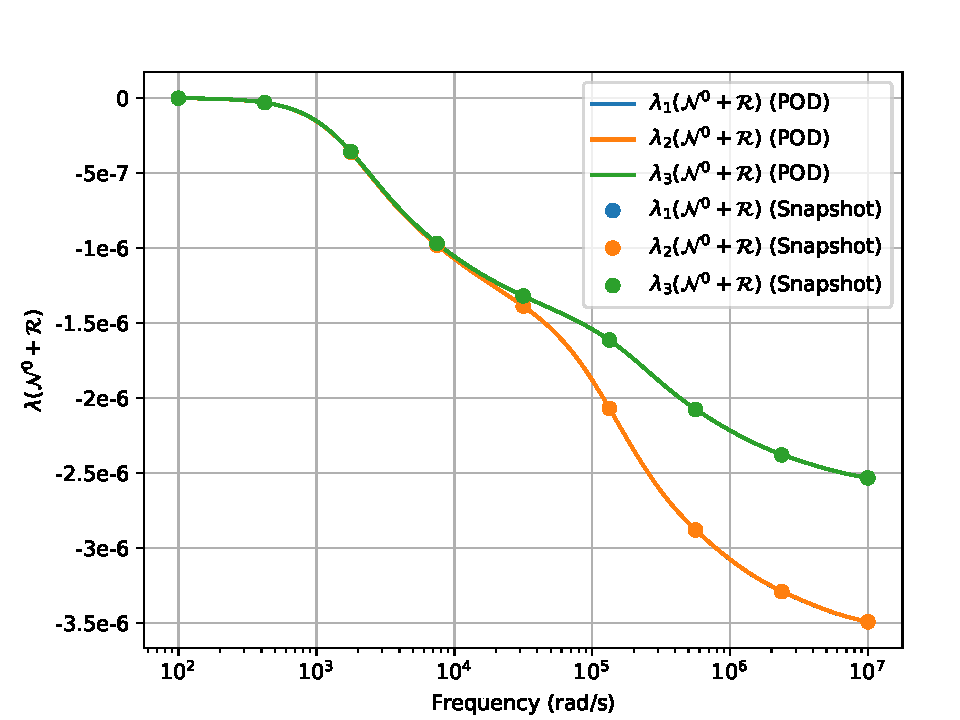
\includegraphics[width=0.48\textwidth, keepaspectratio]{Figures/DualBar/RealEigenvalues.pdf} & 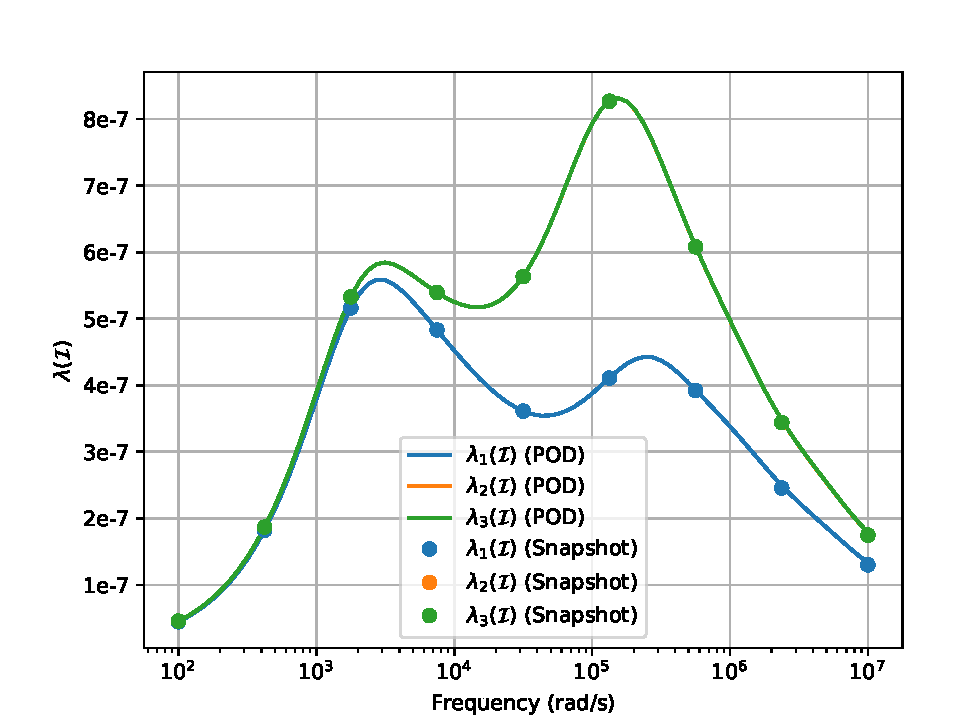
\includegraphics[width=0.48\textwidth, keepaspectratio]{Figures/DualBar/ImaginaryEigenvalues.pdf}\\
\textrm{\footnotesize{(a) A graph showing how $\lambda(\mathcal{N}^0+\mathcal{R})$ changes with frequency.}} & \textrm{\footnotesize{(b) A graph showing how $\lambda(\mathcal{I})$ changes with frequency.}}\\
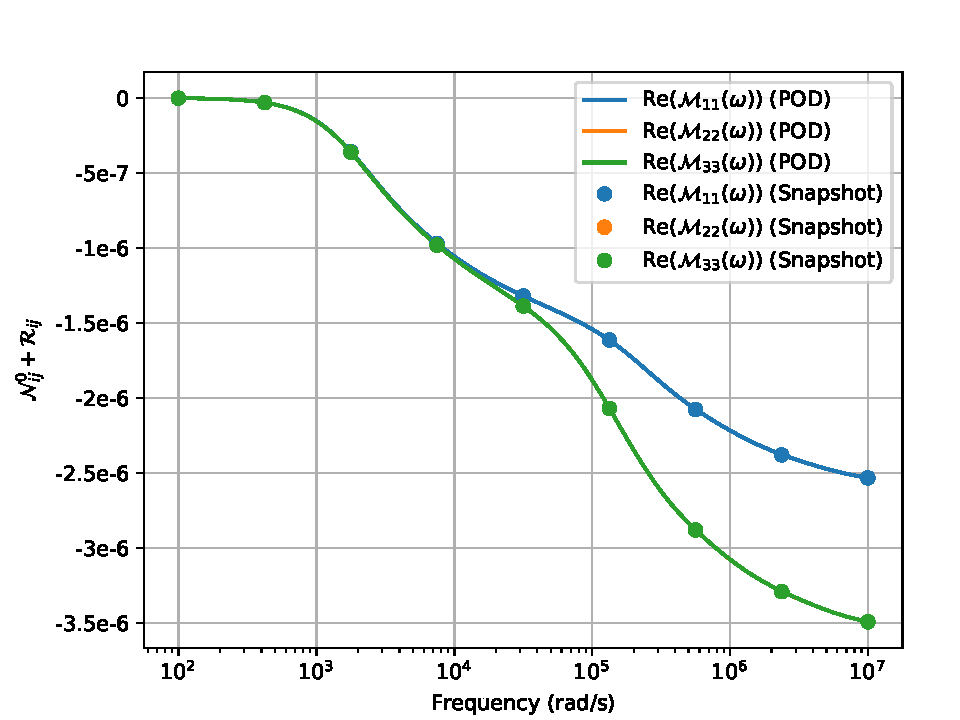
\includegraphics[width=0.48\textwidth, keepaspectratio]{Figures/DualBar/RealTensorCoeficients.pdf} & 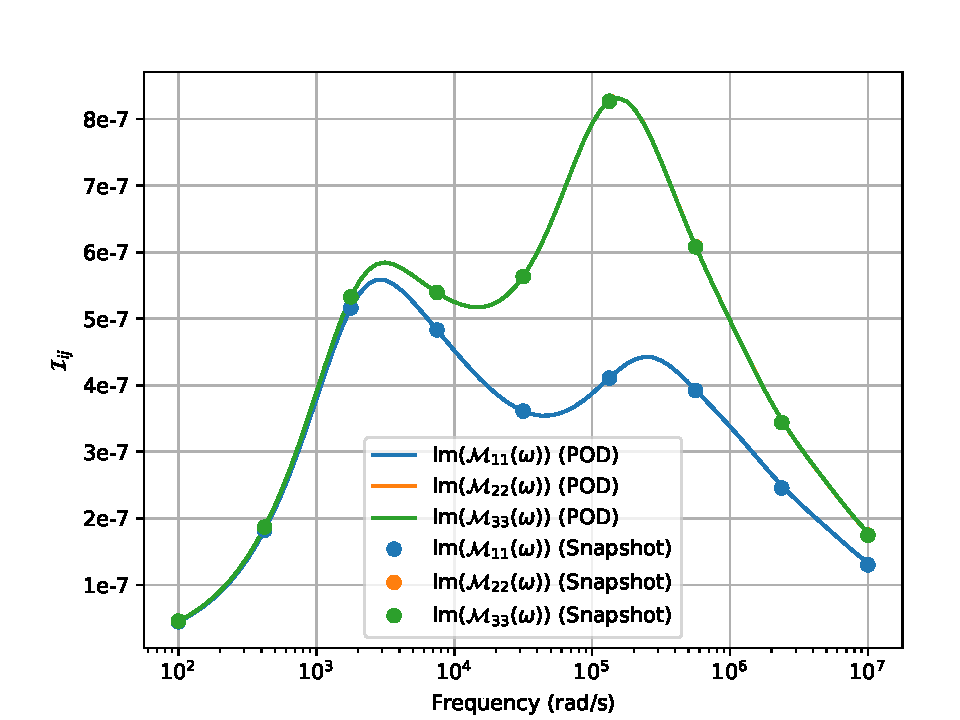
\includegraphics[width=0.48\textwidth, keepaspectratio]{Figures/DualBar/ImaginaryTensorCoeficients.pdf}\\
\textrm{\footnotesize{(c) A graph showing how $\mathcal{N}^0_{ij}+\mathcal{R}_{ij}$ change with frequency.}} & \textrm{\footnotesize{(d) A graph showing how $\mathcal{I}_{ij}$ change with frequency.}}
\end{array}$$
%\begin{figure}\label{LogvsLin}
\caption{Graphs displaying the eigenvalues and tensor coefficients of both the real and imaginary parts for $\mathcal{M}$ calculated using a reduced order frequency sweep for a bar constructed of two regions.}
\label{fig:DualBarOutputs}
\end{figure}
\noindent
In this case, we have chosen to plot only the non-zero coefficients of the tensors by changing the settings in \texttt{PlotterSettings.py}, also, note that even though we have \texttt{EddyCurrentLine = True} no line is produced, this is due to having \texttt{EddyCurrentTest = False} in \texttt{Settings.py}. With this we conclude our example of the bar of two regions, we next consider the case of a rifle shell.
\subsection{Rifle shell casing}\label{sectRifle}
Finally, we consider  $\alpha B$ to the be the rifle shell casing as defined in ~\cite{Rehim2015,LedgerLionheart2016} where $B$ is defined such that $\alpha=0.001$\text{m}. The geometry for $B$ is defined by the \texttt{rifle.geo} file in Figure \ref{fig:rifle.geo}, where $\Omega$ is chosen to be a cube with sides of length 2000 containing the shell $B$, which has material properties $\sigma_*=1.5\times10^7\text{ S/m}$ and $\mu_*=\mu_0$.

\begin{figure}[H]
\begin{center}
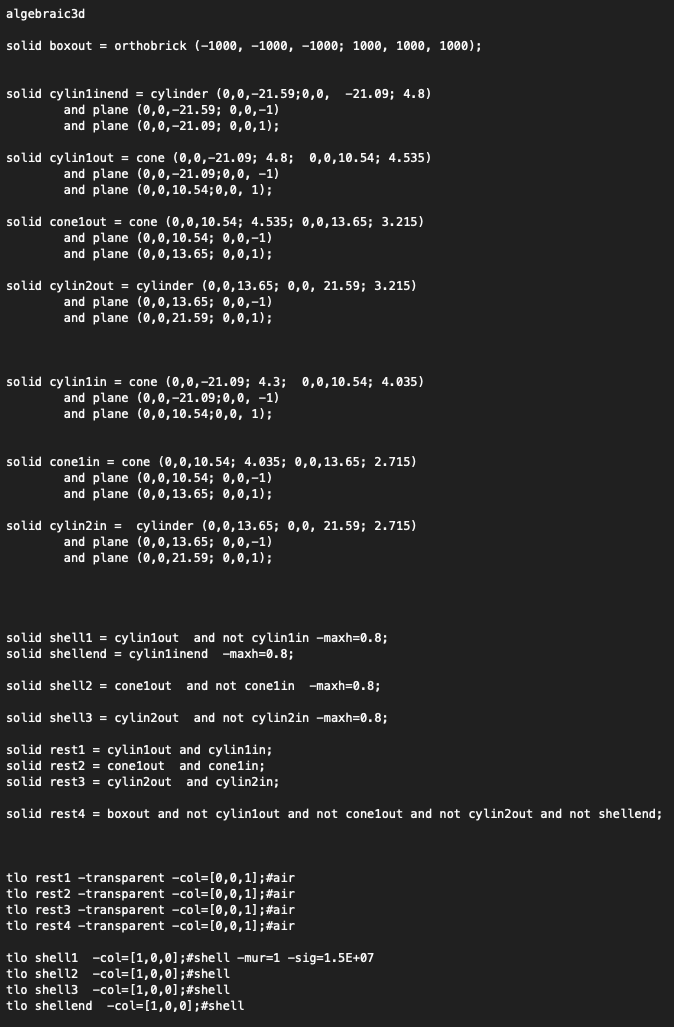
\includegraphics[width=0.55\textwidth]{Figures/rifleInput.png}
\caption{An image showing the \texttt{rifle.geo} file used to simulate the rifle shell casing.}\label{fig:rifle.geo}
\end{center}
\end{figure}
\noindent
To set up this simulation, we used the \texttt{rfle.geo} file show in Figure \ref{fig:rifle.geo} along with the inputs summarised in Table \ref{tab:rifleInputs}.
\begin{table}[H]
\begin{center}
\large{\texttt{main.py}}\normalsize{ }\\\vspace{0.2cm}
\begin{tabular}{!\vrule p{4.5cm}!\vrule p{4.5cm}!\vrule p{4.5cm}!\vrule}
\hline
\texttt{Geometry = "rifle.geo"} & \texttt{alpha = 0.001} & \texttt{MeshSize = 3}\\\hline
\texttt{Order = 3} & \texttt{Start = 1} & \texttt{Finish = 8}\\\hline
\texttt{Points = 81} & \texttt{Single = True} &\texttt{Omega = 100000}\\\hline
\end{tabular}\\
\begin{tabular}{!\vrule p{4.5cm}!\vrule p{4.5cm}!\vrule}
\texttt{Pod = False} & \texttt{MultiProcessing = True}\\\hline
\end{tabular}
\\\vspace{0.5cm}\large{\texttt{Settings.py}}\normalsize{ }\\\vspace{0.2cm}
\begin{tabular}{!\vrule p{4.5cm}!\vrule p{4.5cm}!\vrule p{4.5cm}!\vrule}
\hline
\texttt{CPUs = 3} & \texttt{BigProblem = False} & \texttt{PODPoints = 13}\\\hline
\texttt{PODTol = 0.0001} & \texttt{OldMesh = False} & \texttt{PlotPod = False}\\\hline
\texttt{PODErrorBars = False} & \texttt{EddyCurrentTest = False} & \texttt{vtk\_output = True}\\\hline
\texttt{Refine\_vtk = False} & \texttt{FolderName = "Default"} & \texttt{Solver = "bddc"}\\\hline
\texttt{epsi = 1e-10} & \texttt{Maxsteps = 1500} & \texttt{Tolerance = 1e-08}\\\hline
\end{tabular}\\
\begin{tabular}{!\vrule p{4.5cm}!\vrule}
\texttt{ngsglobals.msg\_level = 0}\\\hline
\end{tabular}
\caption{A table summarising the inputs for the simulation of a rifle shell casing for a reduced order frequency sweep.}\label{tab:rifleInputs}
\end{center}
\end{table}
%\begin{table}[H]
%\begin{center}
%\begin{tabular}{!\vrule l!\vrule l!\vrule l!\vrule}
%\hline
%\texttt{Geometry = "rifle.geo"} & \texttt{Pod = True} & \texttt{EddyCurrentTest = False}\\\hline
%\texttt{alpha = 0.001} & \texttt{MultiProcessing = True} & \texttt{vtk\_output = False}\\\hline
%\texttt{MeshSize = 3} & \texttt{CPUs = 4} & \texttt{Refine\_vtk = False}\\\hline
%\texttt{Order = 3} & \texttt{BigProblem = False} & \texttt{FolderName = "Default"}\\\hline
%\texttt{Start = 1} & \texttt{PODPoints = 9} & \texttt{Solver = "bddc"}\\\hline
%\texttt{Finish = 9} & \texttt{PODTol = 0.0001} & \texttt{epsi = 1e-10}\\\hline
%\texttt{Points = 81} & \texttt{OldMesh = False} & \texttt{Maxsteps = 1500}\\\hline
%\texttt{Single = False} & \texttt{PlotPod = True} & \texttt{Tolerance = 1e-08}\\\hline
%\texttt{Omega = 133.5} & \texttt{PODErrorBars = False} & \texttt{ngsglobals.msg\_level = 0}\\\hline
%\end{tabular}
%\caption{A table summarising the inputs for the simulation of a rifle shell casing for a reduced order frequency sweep.}\label{tab:rifleInputs}
%\end{center}
%\end{table}
\noindent
This means our interest lies in computing the charcterisation for $\alpha B=0.001B$ at 81 frequencies in the range $10^1\leq\omega\leq10^9\text{ rad/s}$. Furthermore, the inputs lead to a mesh of 80013 elements and a discretisation of $p=3$. In this case, a POD technique using  $9$ snapshots chosen logarithmically (following the approach described in Section \ref{sectmain.py}) is used  to create to create the ROM. 
On a 2012 iMac with a 2.9GHz quad core i5 processor with 16 Gb 1600 MHz DDR3 memory the computation takes 24 minutes and 46 seconds using 4 CPUs.

The inputs of \texttt{PlotterSettings.py} are summarised in Table \ref{tab:riflePlotterInputs} leading to  the results shown  in Figure \ref{fig:rifleOutputs}.
\begin{table}[H]
\begin{center}
\begin{tabular}{!\vrule l!\vrule l!\vrule}
\hline
\texttt{EigsToPlot = [1,2,3]}  & \texttt{TensorsToPlot = [1,4,6]} \\\hline
\texttt{MainLineStyle = "-"} & \texttt{MainMarkerSize = 4} \\\hline
\texttt{SnapshotLineStyle = "o"} & \texttt{SnapshotMarkerSize = 6} \\\hline
\texttt{ErrorBarLineStyle = "--"} & \texttt{ErrorBarMarkerSize = 4} \\\hline
\texttt{Title = False} &  \texttt{EddyCurrentLine = False}\\\hline
\end{tabular}
\caption{A table summarising the inputs for the plots produced by the simulation of a rifle shell casing using a reduced order frequency sweep.}\label{tab:riflePlotterInputs}
\end{center}
\end{table}
\begin{figure}[H]
$$\begin{array}{cc}
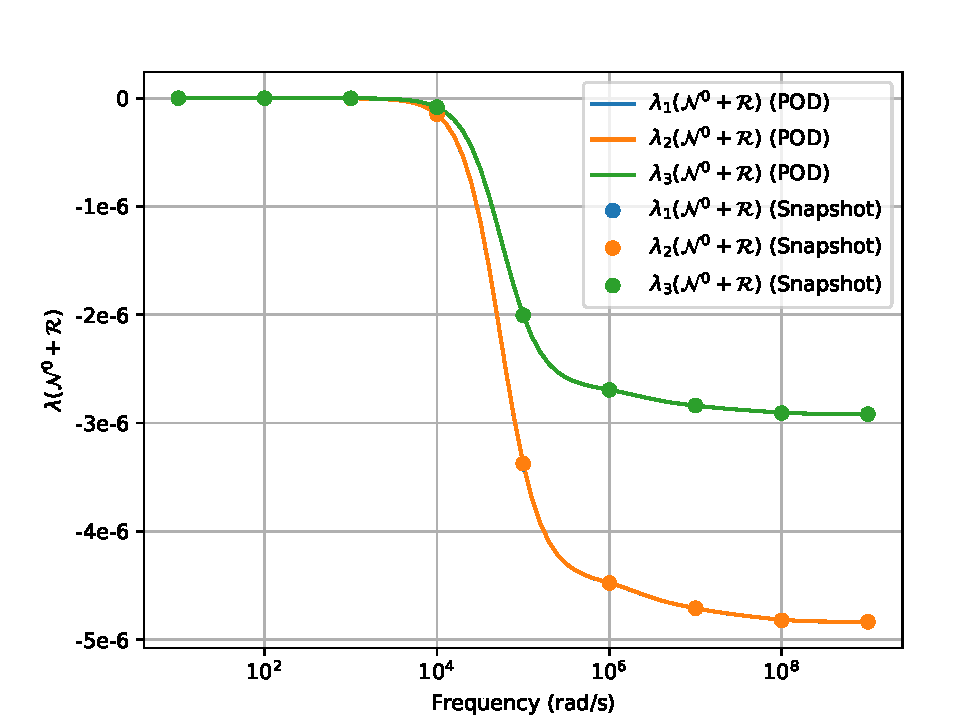
\includegraphics[width=0.48\textwidth, keepaspectratio]{Figures/rifle/RealEigenvalues.pdf} & 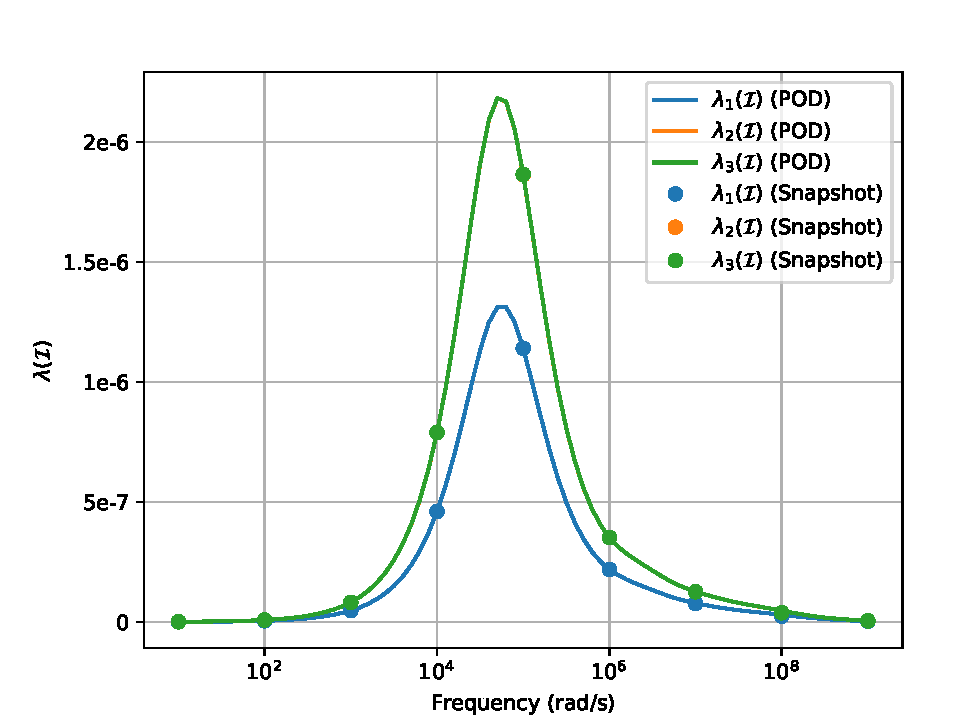
\includegraphics[width=0.48\textwidth, keepaspectratio]{Figures/rifle/ImaginaryEigenvalues.pdf}\\
\textrm{\footnotesize{(a) A graph showing how $\lambda(\mathcal{N}^0+\mathcal{R})$ changes with frequency.}} & \textrm{\footnotesize{(b) A graph showing how $\lambda(\mathcal{I})$ changes with frequency.}}\\
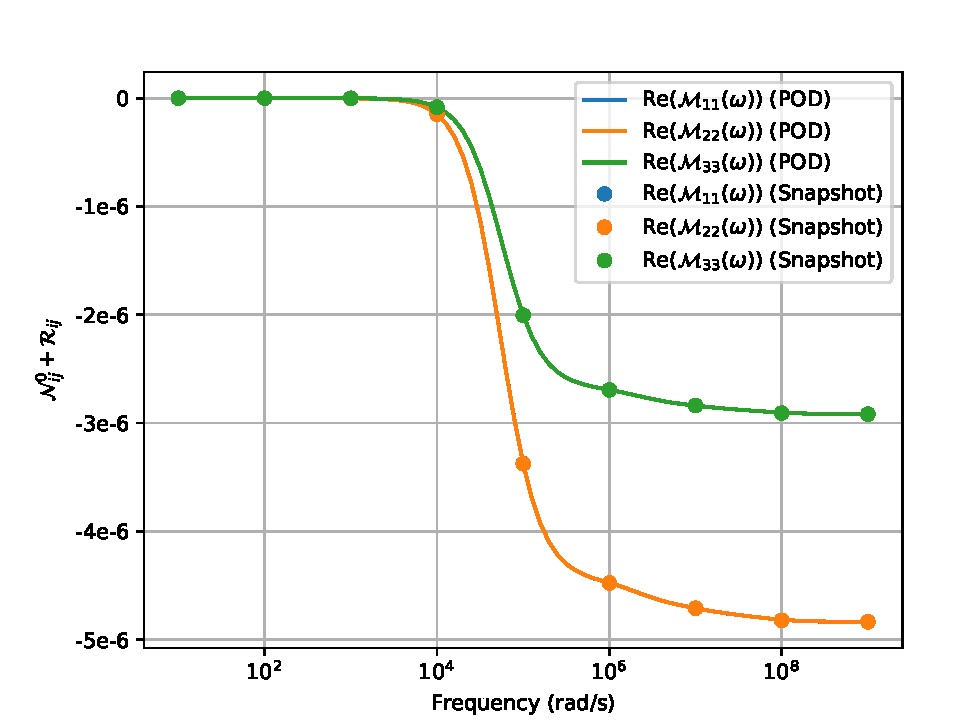
\includegraphics[width=0.48\textwidth, keepaspectratio]{Figures/rifle/RealTensorCoeficients.pdf} & 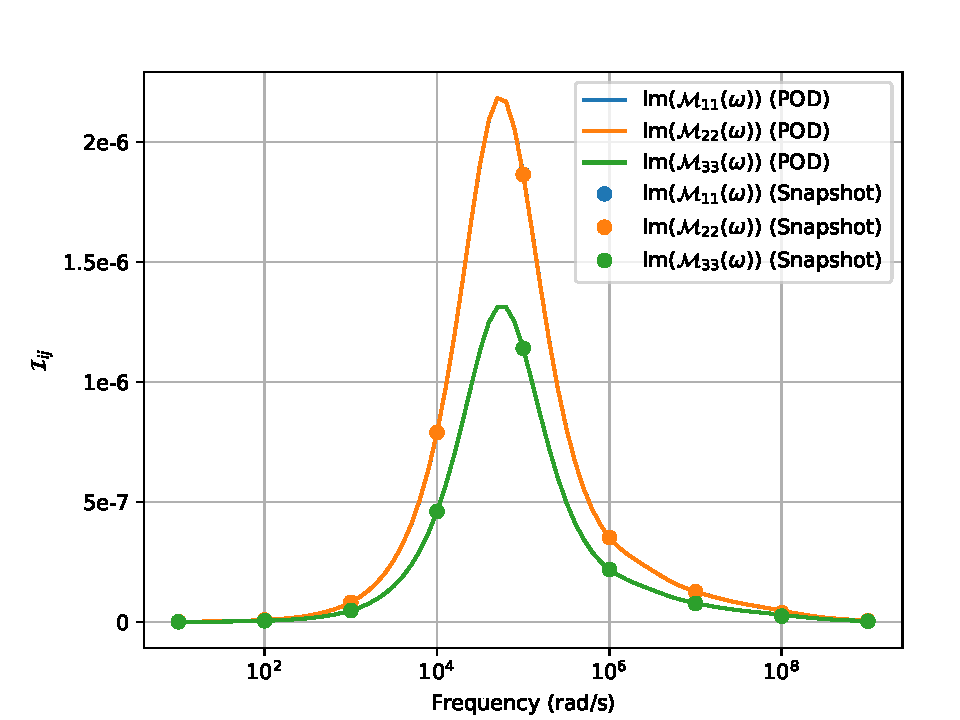
\includegraphics[width=0.48\textwidth, keepaspectratio]{Figures/rifle/ImaginaryTensorCoeficients.pdf}\\
\textrm{\footnotesize{(c) A graph showing how $\mathcal{N}^0_{ij}+\mathcal{R}_{ij}$ change with frequency.}} & \textrm{\footnotesize{(d) A graph showing how $\mathcal{I}_{ij}$ change with frequency.}}
\end{array}$$
%\begin{figure}\label{LogvsLin}
\caption{Graphs displaying the eigenvalues and tensor coefficients of both the real and imaginary parts for $\mathcal{M}$ calculated using a reduced order frequency sweep for a rifle shell casing.}
\label{fig:rifleOutputs}
\end{figure}
\noindent
Once again we have only plotted the non-zero tensor coefficients. In Figure \ref{fig:rifleOutputs} (c) we note that the curve could be improved  around $\omega=10^6$ , although is still  `acceptable' if compared to the full order model. This suggests that we may wish to include some more additional snapshots in the reduced order model. Nevertheless, this  81 point frequency sweep for an object $\alpha B$ discretized by 80013 element mesh with $p=3$ using the POD is computed in considerably less time than the corresponding full order model. We will finally show one more example of the rifle shell casing where a \texttt{.vtk} file is produced, the inputs for this can be seen in Figure \ref{tab:riflevtk}.

\begin{table}[H]
\begin{center}
\large{\texttt{main.py}}\normalsize{ }\\\vspace{0.2cm}
\begin{tabular}{!\vrule p{4.5cm}!\vrule p{4.5cm}!\vrule p{4.5cm}!\vrule}
\hline
\texttt{Geometry = "rifle.geo"} & \texttt{alpha = 0.001} & \texttt{MeshSize = 3}\\\hline
\texttt{Order = 3} & \texttt{Start = 1} & \texttt{Finish = 8}\\\hline
\texttt{Points = 81} & \texttt{Single = True} &\texttt{Omega = 100000}\\\hline
\end{tabular}\\
\begin{tabular}{!\vrule p{4.5cm}!\vrule p{4.5cm}!\vrule}
\texttt{Pod = False} & \texttt{MultiProcessing = True}\\\hline
\end{tabular}
\\\vspace{0.5cm}\large{\texttt{Settings.py}}\normalsize{ }\\\vspace{0.2cm}
\begin{tabular}{!\vrule p{4.5cm}!\vrule p{4.5cm}!\vrule p{4.5cm}!\vrule}
\hline
\texttt{CPUs = 3} & \texttt{BigProblem = False} & \texttt{PODPoints = 13}\\\hline
\texttt{PODTol = 0.0001} & \texttt{OldMesh = False} & \texttt{PlotPod = False}\\\hline
\texttt{PODErrorBars = False} & \texttt{EddyCurrentTest = False} & \texttt{vtk\_output = True}\\\hline
\texttt{Refine\_vtk = False} & \texttt{FolderName = "Default"} & \texttt{Solver = "bddc"}\\\hline
\texttt{epsi = 1e-10} & \texttt{Maxsteps = 1500} & \texttt{Tolerance = 1e-08}\\\hline
\end{tabular}\\
\begin{tabular}{!\vrule p{4.5cm}!\vrule}
\texttt{ngsglobals.msg\_level = 0}\\\hline
\end{tabular}
\caption{A table summarising the inputs for the simulation of a rifle shell casing for a single frequency with a vtk output.}\label{tab:riflevtk}
\end{center}
\end{table}
%\begin{table}[H]
%\begin{center}
%\large{\texttt{main.py}}\normalsize{ }\\\vspace{0.2cm}
%\begin{tabular}{!\vrule l!\vrule l!\vrule l!\vrule}
%\hline
%\texttt{Geometry = "rifle.geo"} & \texttt{Pod = False} & \texttt{EddyCurrentTest = False}\\\hline
%\texttt{alpha = 0.001} & \texttt{MultiProcessing = True} & \texttt{vtk\_output = True}\\\hline
%\texttt{MeshSize = 3} & \texttt{CPUs = 3} & \texttt{Refine\_vtk = False}\\\hline
%\texttt{Order = 3} & \texttt{BigProblem = False} & \texttt{FolderName = "Default"}\\\hline
%\texttt{Start = 1} & \texttt{PODPoints = 13} & \texttt{Solver = "bddc"}\\\hline
%\texttt{Finish = 8} & \texttt{PODTol = 0.0001} & \texttt{epsi = 1e-10}\\\hline
%\texttt{Points = 81} & \texttt{OldMesh = False} & \texttt{Maxsteps = 1500}\\\hline
%\texttt{Single = True} & \texttt{PlotPod = False} & \texttt{Tolerance = 1e-08}\\\hline
%\texttt{Omega = 100000} & \texttt{PODErrorBars = False} & \texttt{ngsglobals.msg\_level = 0}\\\hline
%\end{tabular}
%\caption{A table summarising the inputs for the simulation of a rifle shell casing for a single frequency with a vtk output.}\label{tab:riflevtk}
%\end{center}
%\end{table}
\noindent
These inputs compute the characterisation for $\alpha B = 0.001B$, at $\omega = 10^5$. The inputs lead to a mesh of 80013 elements with $p=3$ with a final vtk output file size of 33.8 MB which has been used to produce the following image of the eddy-currents in paraview displayed in Figure \ref{fig:riflevtk}. The \texttt{rifle.vtk} file stores 7 fields, which can be seen in Table \ref{tab:riflevtkoutput}.
\begin{table}[H]
\begin{center}
\begin{tabular}{!\vrule l!\vrule l!\vrule l!\vrule}
\hline
 Re(i$\omega\sigma_{\alpha}\bm{\theta}^{(1)}_1$) & Re(i$\omega\sigma_{\alpha}\bm{\theta}^{(1)}_2$) & Re(i$\omega\sigma_{\alpha}\bm{\theta}^{(1)}_3$) \\\hline
 Im(i$\omega\sigma_{\alpha}\bm{\theta}^{(1)}_1$) & Im(i$\omega\sigma_{\alpha}\bm{\theta}^{(1)}_2$) & Im(i$\omega\sigma_{\alpha}\bm{\theta}^{(1)}_3$) \\\hline
\end{tabular}\\
%\shifttext{-1.4pt}{
%\resizebox{2.5cm}{!}{
\begin{tabular}{!\vrule l!\vrule}
\hspace{0.31cm} Object \hspace{0.32cm}\textcolor{white}{,}\\\hline
\end{tabular}%}%}
\caption{A table summarising the outputs saved in the \texttt{.vtk} output file.}\label{tab:riflevtkoutput}
\end{center}
\end{table}
\noindent
These are the real and imaginary parts of the eddy-currents for each or the three solutions along with the parameter Object. The parameter Object corresponds to a cut-off parameter, which is defined as
\begin{equation*}
\chi ( {\bm \xi}) : = \left \{ \begin{array}{ll} 
1 & {\bm \xi} \in B \\
0 & \text{otherwise}.
\end{array} \right .
\end{equation*}
%This Object parameter refers to the conducting regions and non-conducting regions (the regions tagged as air in the \texttt{.geo} file) of the domain and take a value of 1 in the conducting regions and 0 in the non-conducting regions.
This allows the user to apply a threshold filter using Object to remove the outer domain an example of which can be seen in Figure \ref{fig:riflethreshold}. The user may use this to show the eddy currents corresponding to $\text{Re}( \im \omega \sigma_{\alpha} {\bm \theta}_1^{(1)} )$ for just $B$ which can be seen in Figure \ref{fig:riflevtk}.
\begin{figure}[H]
\begin{center}
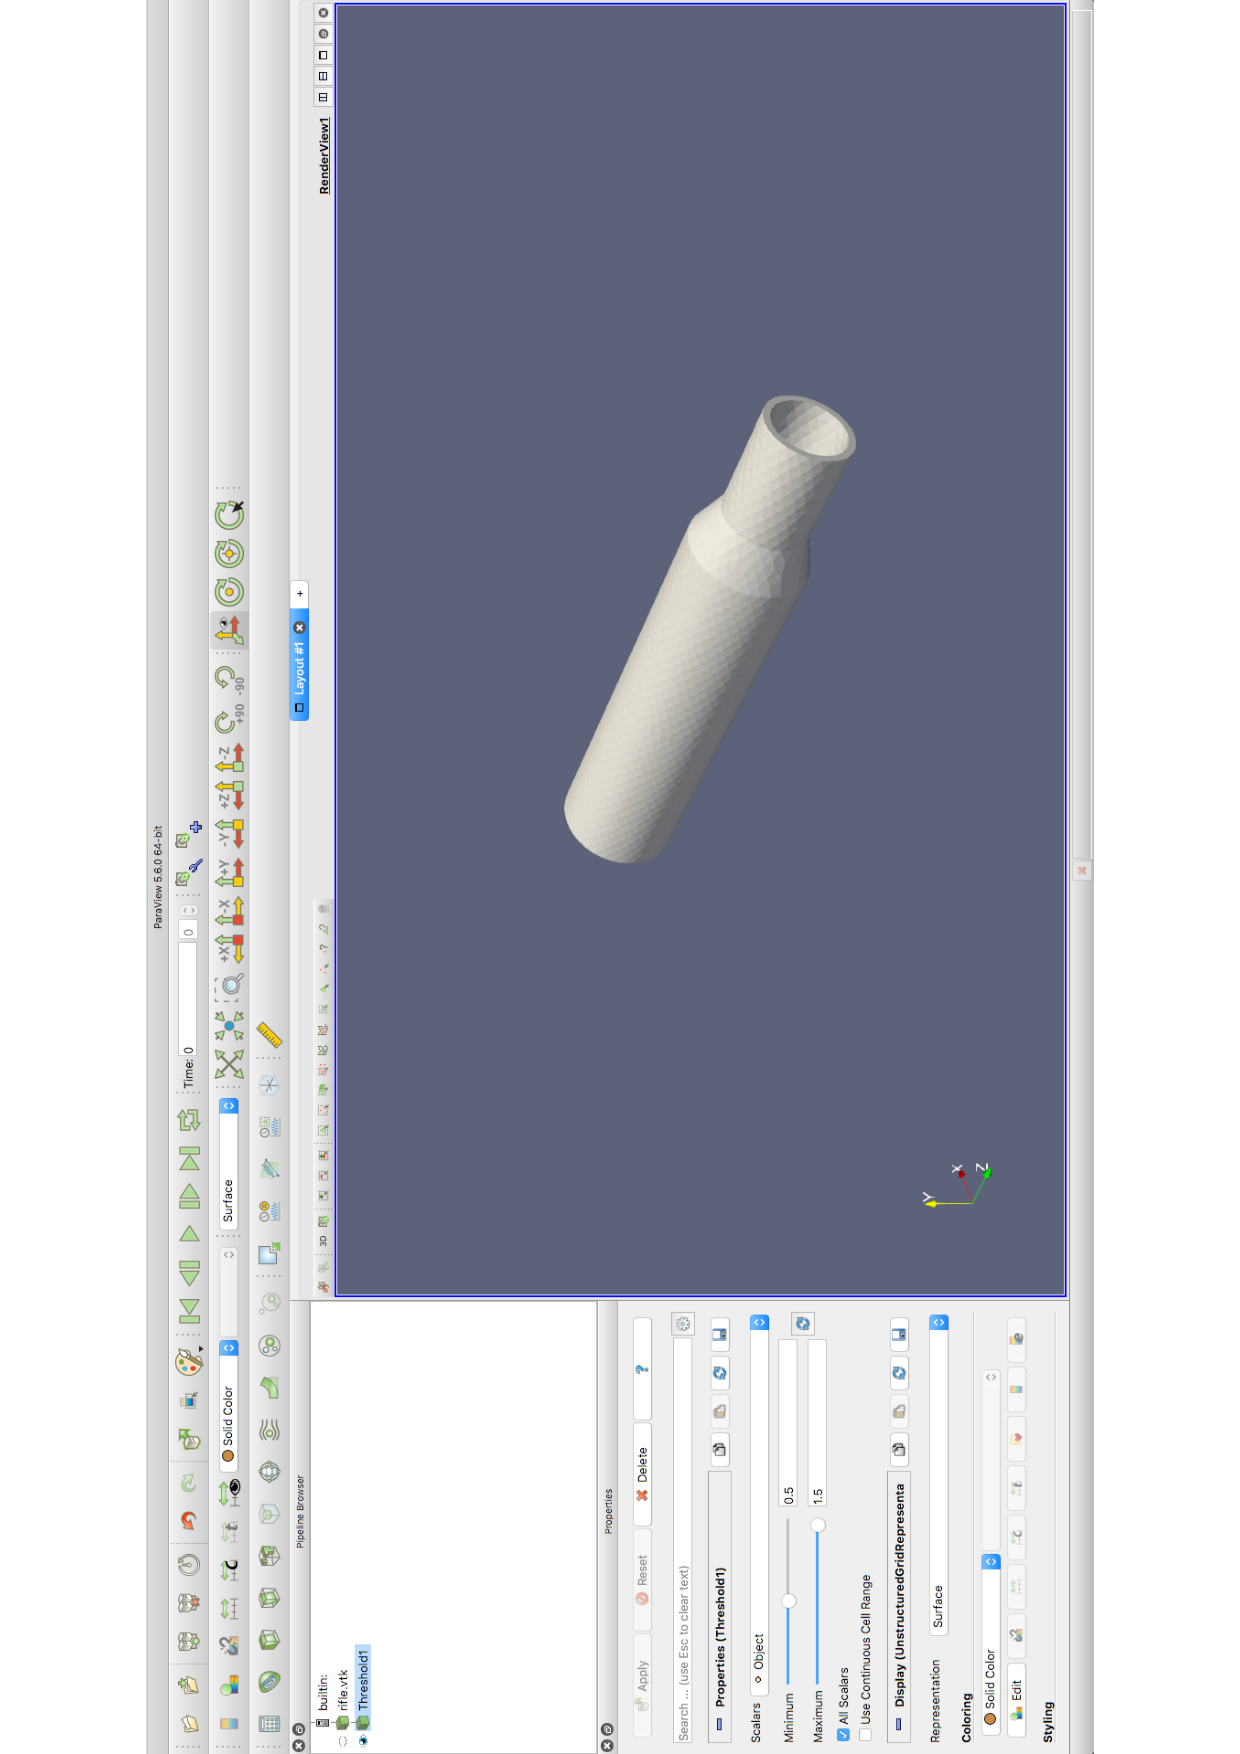
\includegraphics[width=0.95\textwidth]{Figures/riflethreshold}
\caption{An image showing the use of the object parameter in a rifle shell casing.}\label{fig:riflethreshold}
\end{center}
\end{figure}
%To produce the image in Figure \ref{fig:riflevtk} we have applied a threshold filter to display only the rifle shell casing, then we have displayed Re(i$\omega\sigma_*\bm{\theta}^{(1)}_1$).
\begin{figure}[H]
\begin{center}
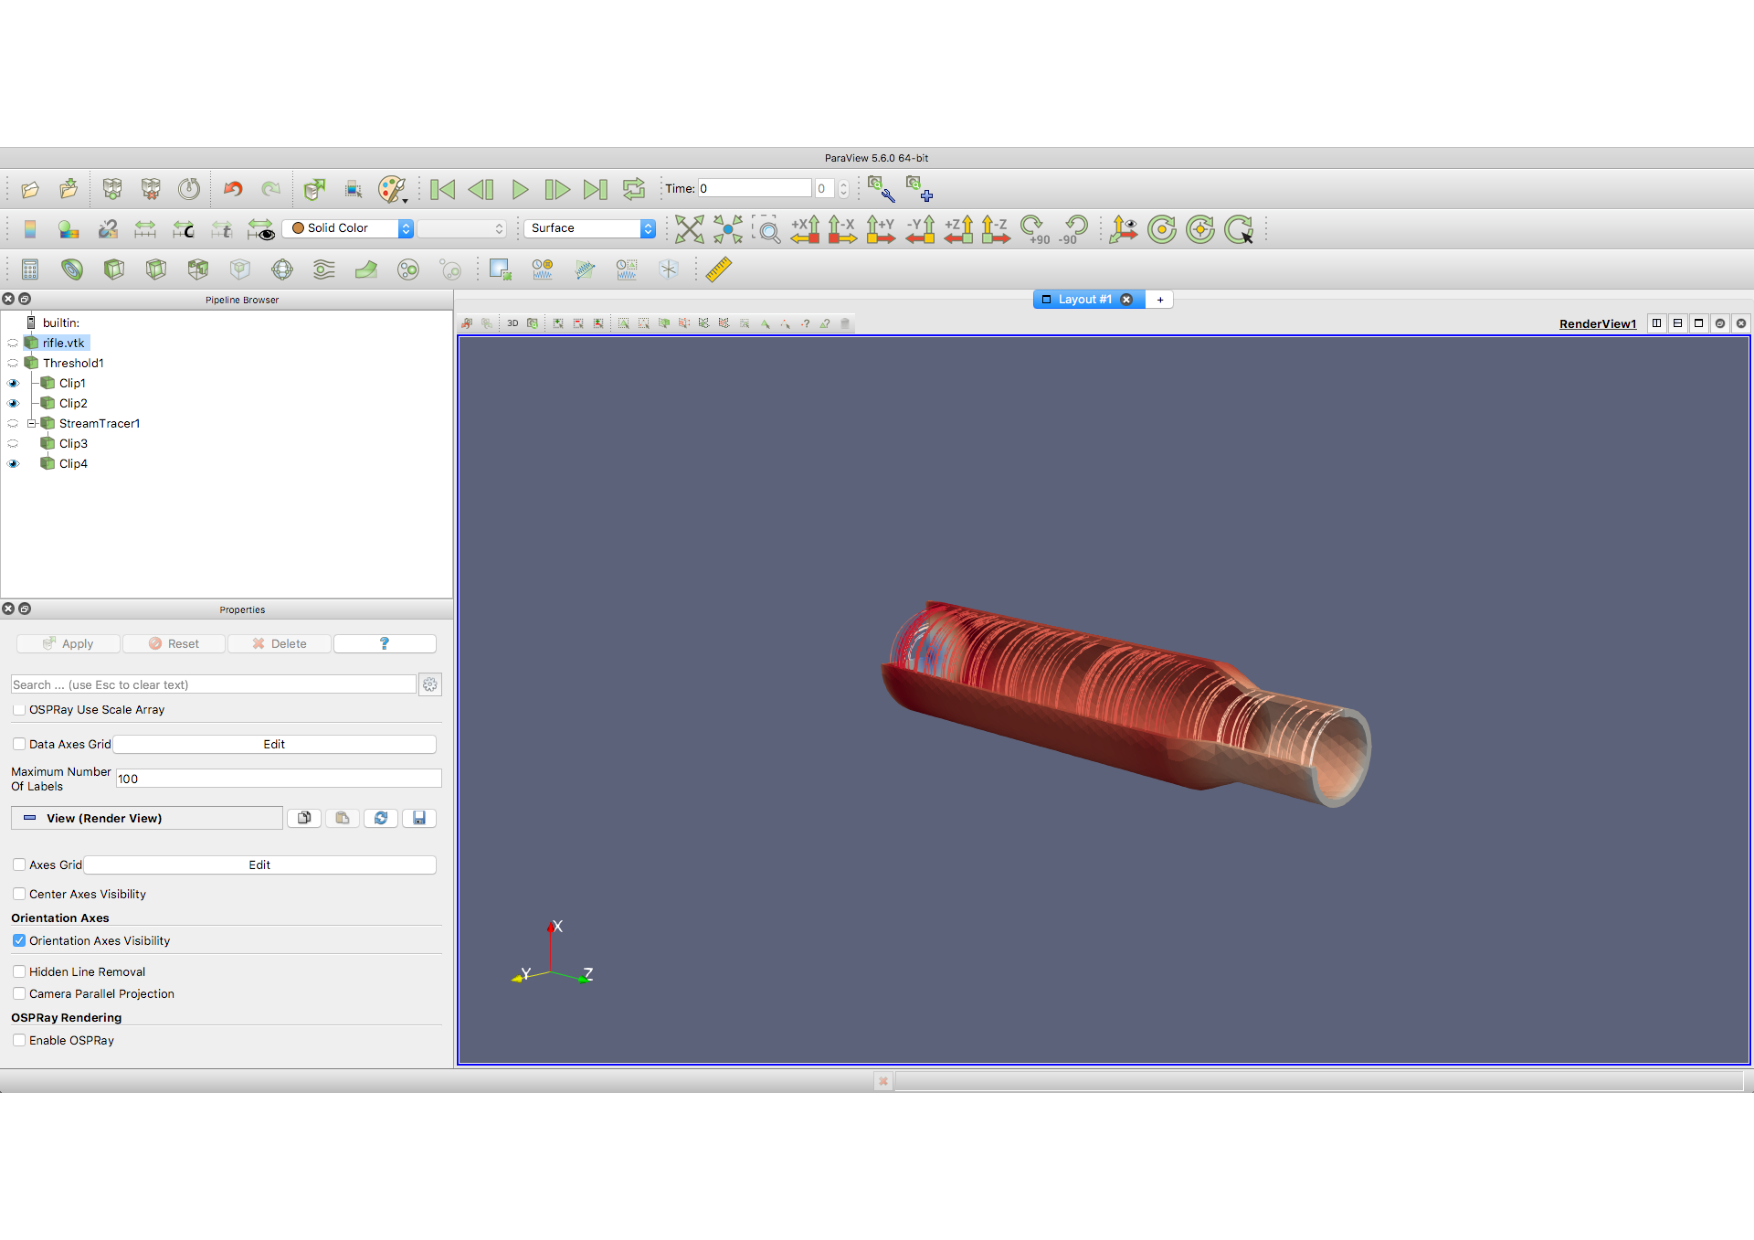
\includegraphics[width=0.95\textwidth]{Figures/rifleshell.pdf}
\caption{An image showing the eddy-currents in a rifle shell casing with $\omega=10^5$ rad/s.}\label{fig:riflevtk}
\end{center}
\end{figure}
\noindent
With this we conclude the examples section. Along with the \texttt{.geo} files for the examples which have been discussed in this article, there are a selection of other \texttt{.geo} files which are included with the download of the code.

%\section{Known issues}\label{Issues}

%There is currently 1 known issues with the \texttt{MPT-Calculator} which we are currently working to resolve.
%\begin{itemize}
%\item There is an occasional failure whilst running simulations for points in a frequency sweep which is due to an issue with NGSolve. If this happens you need to rerun the sweep.

%\item Currently whilst using NGSolve-6.2.1910 there is an issue with producing off diagonal coefficients for the Imaginary Tensor from the reduced order model. This can be fixed by setting \texttt{ImagTensorFullOrd\\erCalc = True}, which can be found in the file \texttt{Functions/PODFunctions.py}. Please note that this will slow down the simulation slightly.
%\end{itemize}

\section{Citation}

If you use the tool, please refer to it in your work by citing the references

\begin{itemize}
\item	~\cite{wilsonledger2019} B. A. Wilson and P. D. Ledger, Efficient computation of the magnetic polarizabiltiy tensor spectral signature using pod. International Journal for Numerical Methods in Engineering 122, 1940-1963, 2021. %\href{https://arxiv.org/abs/2001.07629}

\item~\cite{ledger2020identification} P. D. Ledger, B. A. Wilson, A. A. S. Amad, W. R. B. Lionheart Identification of meallic objects using spectral MPT signatures: Object characterisation and invariants. International Journal for Numerical Methods in Engineering. Accepted Author Manuscript, 2021. %\href{https://onlinelibrary.wiley.com/doi/10.1002/nme.6688}

\item ~\cite{LedgerLionheart2019}, P. D. Ledger and W. R. B. Lionheart, The spectral properties of the magnetic polarizability tensor for metallic object characterisation, Math Meth Appl Sci., 43, 78-113, 2020,

\item ~\cite{LedgerLionheart2018} P. D. Ledger and W. R. B. Lionheart,  An explicit formula for the magnetic polarizability tensor for object characterization, {IEEE} Trans Geosci Remote Sens., 56(6), 3520-3533, 2018.



\end{itemize}

as well as those of \texttt{NGSolve}:

\begin{itemize}
\item \cite{NGSolve} J. Sch\"oberl, C++11 Implementation of Finite Elements in NGSolve, ASC Report 30/2014, Institute for Analysis and Scientific Computing, Vienna University of Technology, 2014.
%%
\item ~\cite{zaglmayrphd} S. Zaglmayr, High Order Finite Elements for Electromagnetic Field Computation, PhD Thesis, Johannes Kepler University Linz, 2006 
%%
\item \cite{netgendet},
J. {Sch\"oberl}, NETGEN - An advancing front 2D/3D-mesh generator based on abstract rules, Computing and Visualization in Science, 1(1), 41-52, 1997.
%%0
\end{itemize}







































